\documentclass[12pt, twoside,openright,a4paper,papersize,uplatex,dvipdfmx, report]{jsbook}
% uplatex オプションを指定し、ユニコード対応に。ただだし、uplatex でコンパイルすること。

% 修論本体と表紙で共通で必要となる設定
% jsbookで余白が広すぎるのを直す
% 参照 https://oku.edu.mie-u.ac.jp/~okumura/jsclasses/
\setlength{\textwidth}{\fullwidth}
\setlength{\evensidemargin}{\oddsidemargin}
\addtolength{\textwidth}{-5truemm}
\addtolength{\oddsidemargin}{5truemm}

% 同梱の ISEE 用の表紙テンプレ
\usepackage{thesis_cover}

% OTF フォントを使えるようにし、複数のウェイトも使用可能にする。
% これがないと、Mac のヒラギノ環境で使われる角ゴが太すぎてみっともない。
\usepackage[deluxe]{otf}
% OT1→T1に変更し、ウムラウトなどを PDF 出力で合成文字ではなくす
\usepackage[T1]{fontenc}
% uplatex の場合に必要な処理 
\usepackage[utf8]{inputenc} % エンコーディングが UTF8 であることを明示する。
\usepackage[prefernoncjk]{pxcjkcat} % アクセントつきラテン文字を欧文扱いにする
% Helvetica と Times を sf と rm のそれぞれで使う。
% default だとバランスが悪いので、日本語に合わせて文字の大きさを調整する。
\usepackage[scaled=1.05,helvratio=0.95]{newtxtext}
% 色
\usepackage[dvipdfmx]{color}
% 行番号を表示する。
\usepackage{lineno}

% latexdiff
% 実際の修論には入れる必要なし
%DIF PREAMBLE EXTENSION ADDED BY LATEXDIFF
%DIF UNDERLINE PREAMBLE %DIF PREAMBLE
\RequirePackage[normalem]{ulem} %DIF PREAMBLE
\RequirePackage{color}\definecolor{RED}{rgb}{1,0,0}\definecolor{BLUE}{rgb}{0,0,1} %DIF PREAMBLE
\providecommand{\DIFadd}[1]{{\protect\color{blue}\uwave{#1}}} %DIF PREAMBLE
\providecommand{\DIFdel}[1]{{\protect\color{red}\sout{#1}}}                      %DIF PREAMBLE
%DIF SAFE PREAMBLE %DIF PREAMBLE
\providecommand{\DIFaddbegin}{} %DIF PREAMBLE
\providecommand{\DIFaddend}{} %DIF PREAMBLE
\providecommand{\DIFdelbegin}{} %DIF PREAMBLE
\providecommand{\DIFdelend}{} %DIF PREAMBLE
%DIF FLOATSAFE PREAMBLE %DIF PREAMBLE
\providecommand{\DIFaddFL}[1]{\DIFadd{#1}} %DIF PREAMBLE
\providecommand{\DIFdelFL}[1]{\DIFdel{#1}} %DIF PREAMBLE
\providecommand{\DIFaddbeginFL}{} %DIF PREAMBLE
\providecommand{\DIFaddendFL}{} %DIF PREAMBLE
\providecommand{\DIFdelbeginFL}{} %DIF PREAMBLE
\providecommand{\DIFdelendFL}{} %DIF PREAMBLE
%DIF END PREAMBLE EXTENSION ADDED BY LATEXDIFF


%% 以下追加したpackage
% 画像の取り扱いに必要
\usepackage{graphicx}
% 数式の機能を拡張
\usepackage{amsmath}
\usepackage{bm}
\usepackage{upgreek}
\usepackage{newtxmath,newtxtext}
% コードを表示
\usepackage{listings}
\lstset{
    %プログラム言語(複数の言語に対応,C,C++も可)
    language = Python,
    %背景色と透過度
    backgroundcolor={\color[gray]{.98}},
    %枠外に行った時の自動改行
    breaklines = true,
    %自動改行後のインデント量(デフォルトでは20[pt])	
    breakindent = 10pt,
    %標準の書体
    basicstyle = \ttfamily\scriptsize,
    %コメントの書体
    commentstyle = {\itshape \color[cmyk]{1,0.4,1,0}},
    %関数名等の色の設定
    classoffset = 0,
    %キーワード(int, ifなど)の書体
    keywordstyle = {\bfseries \color[cmyk]{0,1,0,0}},
    %表示する文字の書体
    stringstyle = {\ttfamily \color[rgb]{0,0,1}},
    %枠 "t"は上に線を記載, "T"は上に二重線を記載
    %他オプション:leftline,topline,bottomline,lines,single,shadowbox
    frame = tbrl,
    %frameまでの間隔(行番号とプログラムの間)
    framesep = 5pt,
    %行番号の位置
    numbers = left,
    %行番号の間隔
    stepnumber = 1,
    %行番号の書体
    numberstyle = \tiny,
    %タブの大きさ
    tabsize = 4,
    %キャプションの場所("tb"ならば上下両方に記載)
    captionpos = t
}
% 複数引用
\usepackage{cite}
%\usepackage{natbib}
% 複数図を並べる時のcaption
\usepackage{subcaption}
\usepackage{here}
% 表関連
\usepackage{booktabs}
% 表でセルを複数列で結合する
\usepackage{multicol}
\usepackage{multirow}
% PDF 内で外部リンクや文書内リンクを生成したい場合に使う(好みによる)
\usepackage[dvipdfmx, hidelinks]{hyperref}
\usepackage{url}
% 複数行コメント
\usepackage{comment}
% 番号付き箇条書きのオプション利用
\usepackage{enumerate}
% renewcommandなどはここに
\usepackage{mymacros}
% 目次でsubsectionまで表示
\setcounter{tocdepth}{2}



% 画像の取り扱いに必要
\usepackage{graphicx}
% 数式の機能を拡張
\usepackage{amsmath}
\usepackage{bm}
\usepackage{upgreek}
\usepackage{newtxmath,newtxtext}
% コードを表示
\usepackage{listings}
\lstset{
    %プログラム言語(複数の言語に対応,C,C++も可)
    language = Python,
    %背景色と透過度
    backgroundcolor={\color[gray]{.98}},
    %枠外に行った時の自動改行
    breaklines = true,
    %自動改行後のインデント量(デフォルトでは20[pt])	
    breakindent = 10pt,
    %標準の書体
    basicstyle = \ttfamily\scriptsize,
    %コメントの書体
    commentstyle = {\itshape \color[cmyk]{1,0.4,1,0}},
    %関数名等の色の設定
    classoffset = 0,
    %キーワード(int, ifなど)の書体
    keywordstyle = {\bfseries \color[cmyk]{0,1,0,0}},
    %表示する文字の書体
    stringstyle = {\ttfamily \color[rgb]{0,0,1}},
    %枠 "t"は上に線を記載, "T"は上に二重線を記載
    %他オプション:leftline,topline,bottomline,lines,single,shadowbox
    frame = tbrl,
    %frameまでの間隔(行番号とプログラムの間)
    framesep = 5pt,
    %行番号の位置
    numbers = left,
    %行番号の間隔
    stepnumber = 1,
    %行番号の書体
    numberstyle = \tiny,
    %タブの大きさ
    tabsize = 4,
    %キャプションの場所("tb"ならば上下両方に記載)
    captionpos = t
}
% 複数引用
\usepackage{cite}
%\usepackage{natbib}
% 複数図を並べる時のcaption
\usepackage{subcaption}
\usepackage{here}
% 表関連
\usepackage{booktabs}
% 表でセルを複数列で結合する
\usepackage{multicol}
\usepackage{multirow}
% 行番号を表示する。添削時のみに使い、事務提出版ではコメントアウトする
%\usepackage{lineno}
%\linenumbers
% PDF 内で外部リンクや文書内リンクを生成したい場合に使う(好みによる)
\usepackage[dvipdfmx, hidelinks]{hyperref}
\usepackage{url}
% renewcommandなどはここに
\usepackage{mymacros}
% 目次でsubsectionまで表示
\setcounter{tocdepth}{2}
% 複数行コメント
\usepackage{comment}


% 氏名などの情報が入っているファイル。各自で編集。
%\title{深層学習による消化管腫瘍検出 \\ 〜3次元病理画像解析〜} % 論文題目
\date{2019年1月31日} % 日付(入れたくなければ空欄)
\heisei{31} % 年度
\StudentIdNumber{37-176484} % 学籍番号
\author{松崎  博貴} % 氏名
\seifuku{} % 正本か副本か(このファイルでは変更する必要なし)
% \labname{宇宙線物理学研究室} %
\supervisor{小野寺宏 特任教授} % 指導教員
\cosupervisor{染谷隆夫 教授} % 副指導教員


\begin{document}
% 式番号,図番号,表番号を章ごとの連番にする
\numberwithin{equation}{chapter}
\numberwithin{figure}{chapter}
\numberwithin{table}{chapter}


\frontmatter

%\maketitle
% 上肢機能障害者のためのパーソナルロボットハンドの開発
% Development of Personal Robot Hand for upper limb disable person

% これを入れることでページ番号が表示されない。
%\thispagestyle{empty}

% abstract 環境は jsbook では「概要」と表示してくれないため、手動で表示させる。
% 参照 http://oku.edu.mie-u.ac.jp/tex/mod/forum/discuss.php?d=2121
\begin{center}
  {\LARGE \sf 概要}
\end{center}

近年になって医療データが蓄積されるシステムができてきいる。医療画像をコンピューター上に取り込むようになってから、自動で解析するシステムを構築してきた。今までは、専門医が診断を行う場合は、判断が主観的であること、ミスをする可能性があること、専門化同士でも意見が異なること、実際の臨床現場で医師はたくさんの画像を処理しなくてはいけないので、1枚にかけられる時間が限られていることから、機械による診断支援システムが必要とされている。既存の機械によるルールベースによるシステムでは解析ルール人にバイアスがかかっているということや、画像認識の著しい精度向上があるディープラーニングを利用した方法によって解析する方法に注目されている。またコンピュータの計算性能と、ビッグデータである医療画像を処理する能力が向上した背景と重なって、現在は機械学習による医療画像解析の研究が盛り上がりを見せている。

\tableofcontents
\listoffigures
\listoftables

\mainmatter

% include を使うことで、別ファイルに分割することができます。
\chapter{序論}
\label{chap_intro}
\newpage

\section{研究背景}
\subsection{ロボティクスと深層学習}
ロボティクス技術の向上とともに,様々な分野でロボットが活躍している.特に,医療や福祉といった人間の生活環境下で作業可能なパーソナルロボットの需要の増加は顕著である.しかし,人の生活環境下において完全に自律して動作及び人の補助ができるロボットの実現は困難な状況にある.なぜならば,ロボットが自律行動を行うためには物体や人物の認識,自己位置の認識,そして認識に基づく判断を人の生活環境下で行わなければならないからである.

パーソナルロボットとしてMobile Manipulatorの開発が行われている.Mobile Manipulatorは工場に限定されて使用されているが,これを家庭内でも使用できるように軽く,そして小さくすることで衝突リスクを削減する試みがされている.2018年には,Preferred Networksは室内に散らかった家庭用品を片付けるロボットシステムを発表した\cite{お片づけロボット}.部屋の全自動片付けは従来のロボットシステムでは実現困難であったが,近年の深層学習の発展によって初めて実用的なレベルとなった.物をつかむ,物を置く,動作計画を立てる,人の指示に対応するなど,ロボットが人間の生活空間で仕事をするために必要な物体認識・ロボット制御・音声言語理解技術に最先端の深層学習を用いた結果,ロボットが高速・高精度に動作できるようになった.

しかし,深層学習では多くの計算リソースが必要である.計算リソースとは深層学習を動かすハードウェア(いわゆるPC),特にGPU(Graphical Processor Unit)である.GPUは形状が大きく消費電力も大きいため,高性能なGPUを複数Mobile Manipulatorに搭載することは難しい.そこでCloudネットワークを利用する方法がある.Cloudを介してGPUリソースを使用する.これによりCloudとのインターフェースを有しているデバイスであれば演算性能は低くても推論が可能となり,スマートフォンやノートPC,ラズパイと言った小さなデバイスを使用することができる.しかし常時インターネットに接続している必要があるため,災害時に使用できなくなるという問題がある.一方で,Cloudを使わずLocalで処理を行うEdgeコンピューティングという分野も近年研究開発がされている.Edgeコンピューティングでは一般のPCに搭載するようなGPUを用いず,より小型なデバイス(エッジデバイス)で処理を行うことを目的としており,小型,低消費電力,高精度より高速が求められる.しかし深層学習を使用しているパーソナルロボットは高さ1mと大きく,家庭内などで使用する分には良いが,外に持ち出してどこでも使用するといった事ができない.


\subsection{医療分野におけるロボティクス}
医療分野におけるロボットで一番身近なものと言えば義手である.義手には装飾用義手や能動義手,作業用義手などがあるが,現在主流の筋電電動義手(筋電義手)は,使用者が筋肉を動かすことで筋電位を読み取り直感的な操作を可能にする.しかし,筋電位を用いた義手には訓練が必要でリハビリテーション施設で行う必要があるが,その施設が極めて少ない\cite{リハビリテーション}.また筋電位が上手く出せない患者や,腕そのものはあるが麻痺して動かせない患者に対しては使用できない.さらに非侵襲的な筋電義手では入力信号が限られる.自由度の高い動作を可能にすると重量が大きくなり,使用者の負担が大きくなってしまう.

実際に筆者が茨城県立大学付属病院リハビリテーション科に見学に行った際,義手使用患者へヒアリングをした.
当患者は普段は能動義手を使用しており,リハビリの際に筋電義手も使用している.半年のリハビリでペンを掴むことまでできたという状況である.筋電義手の使用感について聞いたところ,
\begin{itemize}
    \item 筋電義手は重い.
    \item (筋電が)ちゃんと伝わっているかわからない.
    \item 把持力の制御が難しく,(物を)落とすこともよくある.
\end{itemize}
とあまりポジティブな感想はなかった.以上のような課題があるため装着者のニーズを満たす義手がなく,あまり実用的なものが少ないのが現状である.

% 重量の重要性を書く

\section{関連研究}
ここではロボット開発の研究について紹介する.

TOYOTAはHuman Support Robot(HSR)を開発した\cite{HSR}.



机に置いて使うもの
Basic research of upper limb work support system “My Cybernic Robot Arm” for hemiplegic persons\cite{Sankai2018}





強化学習で制御
教師ありで制御


\section{研究目的}
% 筋電入力を避けた
% 自律走行するロボット
% ニーズを明確化する

本研究ではパーソナルロボットを小型化し,義手使用患者や片麻痺患者など上肢機能障害患者を対象としたパーソナルロボットを開発する.義手は常に身につけているように,パーソナルロボットも携帯できるよう小型化し腕の形をしたロボットハンドとする.上肢機能障害者にとってはパーソナルロボットはどんな事態でも動作する必要があるため,今回はCloudは使用せずEdgeで処理を行うこととする.また座って机で作業することが多いため使用場所を机の上に限定し,指定した物をピックアップするタスクを実行できるパーソナルロボットハンドを作製することを目的とする.
 % 背景
\chapter{深層学習とロボット制御}
\label{chap_review}
\newpage

\section{ニューラルネットワーク}\label{sec:NeuralNetwork}
人間の脳にはニューロンと呼ばれる神経細胞が1000億個以上あり,それぞれが複数のニューロンが電気信号によって情報を伝達している.また脳にはシナプスという場所があり,ここで電気信号を細胞体へ受け渡す.細胞体はある閾値以上の電気信号がきた場合に他のニューロンへ電気信号を伝播させる(これを発火と呼ぶ).このようなニューロンとシナプスで行われる演算を模倣したアルゴリズムを作ることができれば,人間のような思考や認識をコンピュータを使って再現できると考えた.そのアルゴリズムがニューラルネットワーク(Neural Network: NN)である.

\subsection{多層パーセプトロン}
ニューラルネットワークは入力層,出力層,隠れ層から構成され,層と層の間にはニューロン同士のつながりの強さを示す重みがある.非線形問題を扱うために1986年Rumelhartによって考案されたのが,パーセプトロンを複数つなぎ合わせ入力と出力以外に隠れた層を持つ多層パーセプトロン(Multi-layer perceptron: MLP)である(\fig {mlp}).ニューラルネットワークで多層パーセプトロンの層を全結合(fully connected: FC)層とも呼ぶ.

\begin{figure}[H]
	\centering
	\begin{minipage}[b]{0.4\columnwidth}
		\centering
		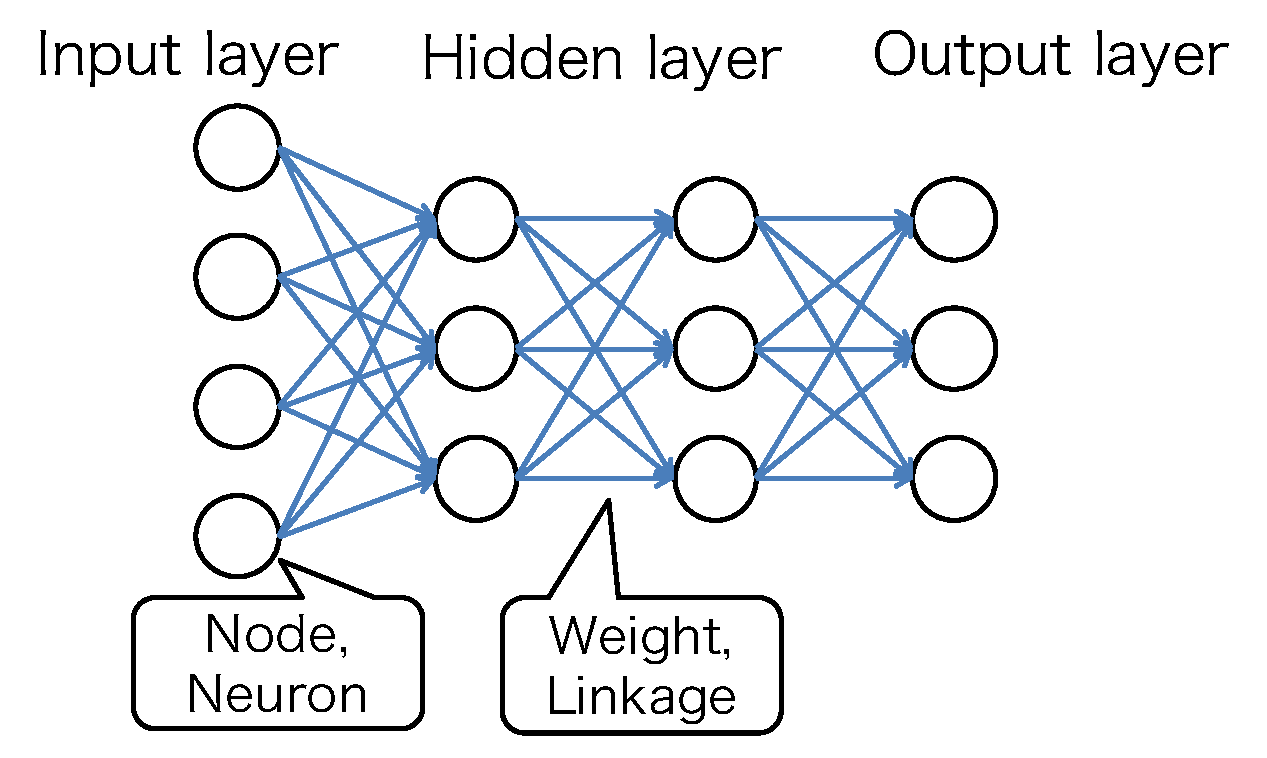
\includegraphics[width=1.2\linewidth]{figure/chapter2/MLP}
		\subcaption{Muti-layer perceptron}
		\label{fig:mlp}
	\end{minipage}
	\begin{minipage}[b]{0.4\columnwidth}
		\centering
		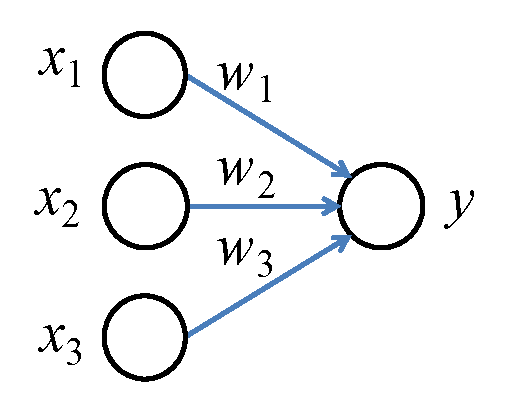
\includegraphics[width=0.7\linewidth]{figure/chapter2/simple_perceptron}
		\subcaption{Simple perceptron}
		\label{fig:perceptron}
	\end{minipage}
	\caption{Architecture of Muti-layer perceptron}
\end{figure}

\fig {mlp}における丸や矢印はそれぞれノード(またはニューロン)と重み(または結合)と呼び,ともに数値である.例えば画像を分類しようと思えば,各ピクセルの画素数を各ノードに入力する.例えば$28 \times 28$pxのグレースケール画像であれば,784個のノードが必要となる.入力データ$\bm {x}$が入力層に入ってくると,その値に重み$\bm {w}$をかけ,活性化関数$H$と呼ばれる関数に通し,結果$\bm{y}$を出力する.ここで,入力$\bm{x}$,重み$\bm{w}$,出力$\bm{y}$を太字で表したが,これらは全てテンソルであり,1つの層にあるノード$x_1, x_2, \cdots x_n$を一括して$\bm {x}$として表記している.

ここで,中間層の1つのノードについて考える.\fig {perceptron}にMLPを構成する1ユニットである単純パーセプトロンを示した.この模式図を数式で表すと次のようになる.
\begin{align}
	y & = H(\bm{w}\bm{x} + \bm{b}) \\
	& = H\left( \sum_{i=1}^3 w_i x_i + b_i \right) 
\end{align}
ここで$\bm{b}$はバイアスと呼ばれ,発火のしやすさを表している.中間層における活性化関数は,\eq {ReLU}に示す正規化線形関数(rectified linear unit: ReLU)と呼ばれる関数)がよく用いられる.
\begin{align}\label{eq:ReLU}
	H(x) = \max \left\lbrace 0, x \right\rbrace = \begin{cases}
	x & (x > 0) \\
	0 & (x \leq 0)
	\end{cases}
\end{align}
この演算を繰り返し出力層に書き出す.ここで,各層の重みの値によって出力結果は異なってくる.

出力層では,ノードの個数は区別したいクラス数分用意する.
各ノードの出力値が各クラスに属している確率を表すように,活性化関数にはソフトマックス関数を用いる(ただし二値分類の場合はシグモイド関数を用いる).ソフトマックス関数は\eq {softmax}で表される.
\begin{align}\label{eq:softmax}
	y_i = \dfrac{\exp(x_i)}{\displaystyle \sum_{k=1}^n \exp(x_k)}
\end{align}
ここで$y_i$は,出力層が全部で$n$個あるとして,$i$番目の出力であることを示す.\eq {softmax}からわかるように,入力の総和に対して1つのノードがどれくらいの値を持つかという割合で表されている.これにより各ノードの出力は確率として解釈できるため,値の一番大きいノードのインデックスを予測ラベルとして見ることができる.


\subsection{畳み込みニューラルネットワーク}
従来の画像認識では,画像から特徴を抽出しそれを識別器にかける手法が主流であった.古典的手法では画像から特徴を抽出するいわゆる特徴量設計が必要で,ここをいかにうまく設計するかがポイントであった.特徴抽出の方法として,HOG\cite{HOG}やSIFT\cite{SIFT},SURF\cite{SURF}などがあり,これらによって抽出した特徴ベクトルをSupport Vector Machine(SVM)\cite{SVM}によって識別することが多かった.

しかし,1998年にLeNetと呼ばれる畳み込みニューラルネットワーク(Convolutional Neural Network: CNN)が提案された\cite{LeNet}.CNNは畳み込み層とプーリング層からなっている.この畳み込みとプーリングの演算を通して,特徴量設計から識別までをend-to-endで行うことができる.

\begin{figure}[H]
	\centering
	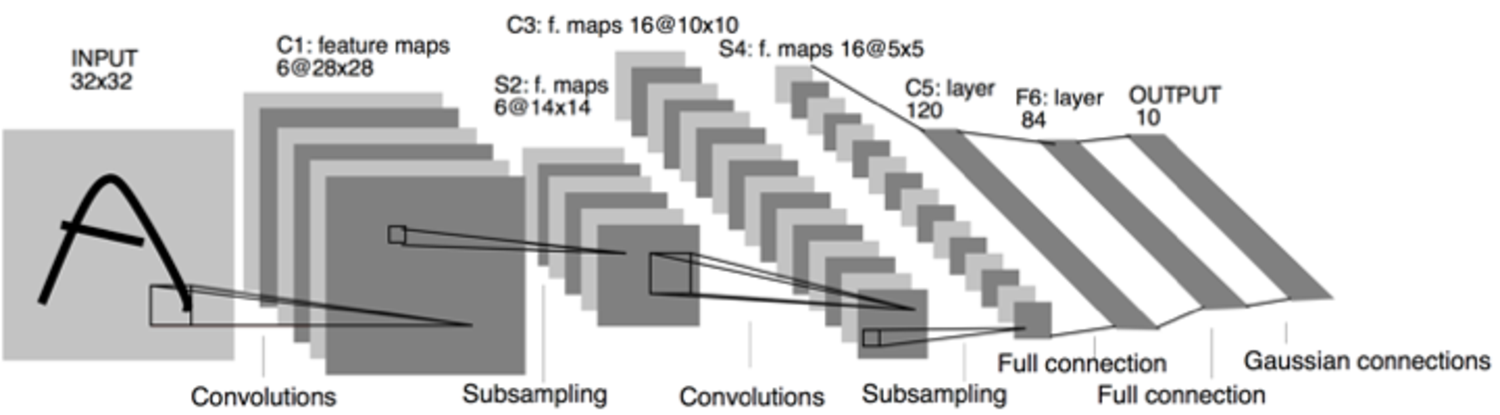
\includegraphics[width=0.7\linewidth]{figure/chapter2/LeNet}
	\caption{Architecture of convolutional neural network\cite{LeNet}}
	\label{fig:LeNet}
\end{figure}


%人間が物体を認識することをコンピュータにも計算させるには,画像の特徴的な部分を切り分けて数値化させる必要がある.例えば,カラー画像の場合,RGBの3色(3チャンネル)を組み合わせた画像で認識をしている.このようなフィルターの畳み込み計算を行うと,フィルターごとに異なった画像の特徴を抽出して数値化する.これが畳み込み(convolution)である.その後,画像のサイズを小さくしてコンピュータが計算コストを減らし,微小な変化に対してロバストになる仕組みしてプーリングという方法を用いる.

畳み込み層では,入力に対してフィルター(カーネルとも呼ばれる)を用意し,\eq {conv}に示す計算を行う.
\begin{align}\label{eq:conv}
	y_{i,j} & = (\bm{K} * \bm{x})_{i,j}\\
	& = \sum_m\sum_n x_{i+m, j+n} K_{m,n}
\end{align}
ここで,$\bm{K}$はフィルター,$\bm{x}$は入力,$y$は出力である.CNNではこの演算の後に活性化関数に通す.これを図で表すと\fig {conv}のようになる.

\begin{figure}[H]
	\centering
	\begin{minipage}{0.45\columnwidth}
		\centering
		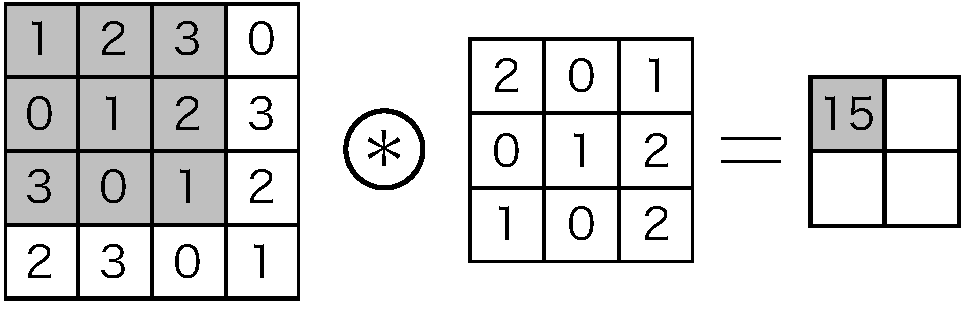
\includegraphics[width=\linewidth]{figure/chapter2/conv_ex1}
		\subcaption{}
		\label{fig:conv_ex1}
	\end{minipage}
	\hspace{10truemm}
	\begin{minipage}{0.45\columnwidth}
		\centering
		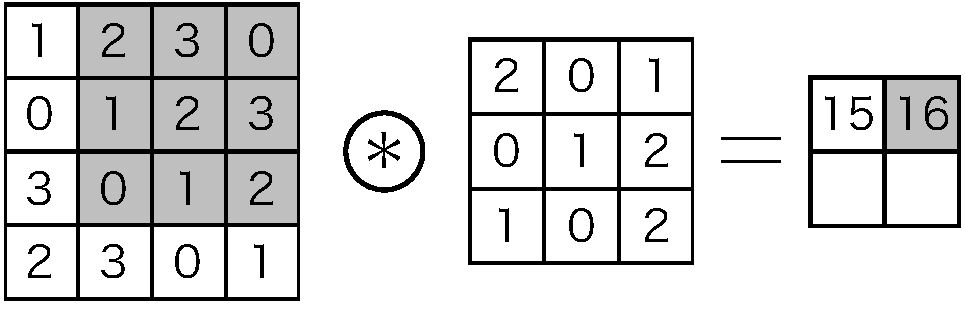
\includegraphics[width=\linewidth]{figure/chapter2/conv_ex2}
		\subcaption{}
		\label{fig:conv_ex2}
	\end{minipage}
	\begin{minipage}{0.45\columnwidth}
		\centering
		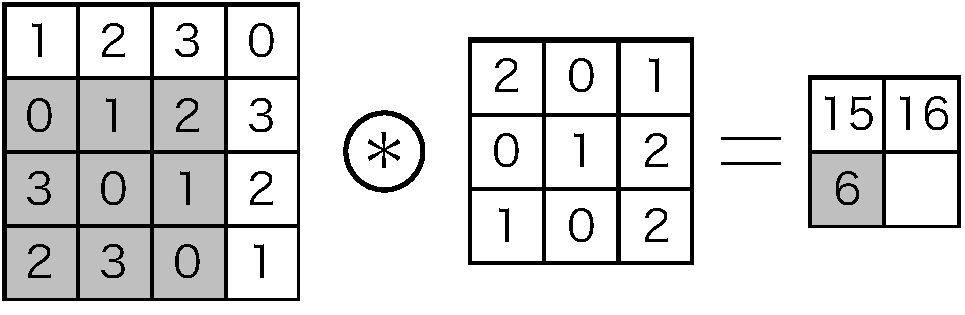
\includegraphics[width=\linewidth]{figure/chapter2/conv_ex3}
		\subcaption{}
		\label{fig:conv_ex3}
	\end{minipage}
	\hspace{10truemm}
	\begin{minipage}{0.45\columnwidth}
		\centering
		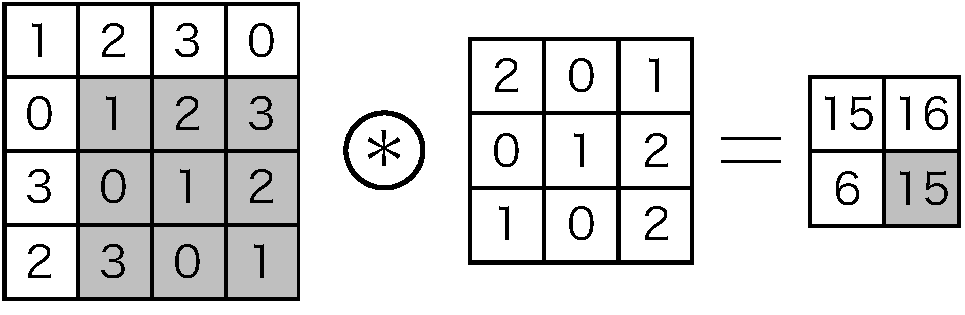
\includegraphics[width=\linewidth]{figure/chapter2/conv_ex4}
		\subcaption{}
		\label{fig:conv_ex4}
	\end{minipage}
	\caption{Operation process of convolution}
	\label{fig:conv}
\end{figure}

\fig {conv}では,フィルターのサイズは$3\times 3$であるが,大きさは任意である($3\times 3$や$5\times 5$, $7\times 7$がよく用いられる).また,フィルターは1マスずつ横にずらして計算を行っている.ずらし方をストライドといい,今回はストライド1である.CNNでは多くの場合,ストライドは1である.
このようなフィルターの畳み込み計算を行うと,フィルターごとに異なった画像の特徴を抽出して数値化することができる.

次にプーリングを行う.ここでは,画像認識で多く用いられる最大値プーリングについて述べる.\fig {maxpooling}に示すように,$2\times 2$のプールサイズを用意した時,その範囲内にある最大値を取る演算である.ストライドはプールサイズと合わせ,プーリングを行った領域と被らないようにすることが一般的である.\fig {maxpooling}ではストライド2である.

\begin{figure}[H]
	\centering
	\begin{minipage}[b]{0.4\columnwidth}
		\centering
		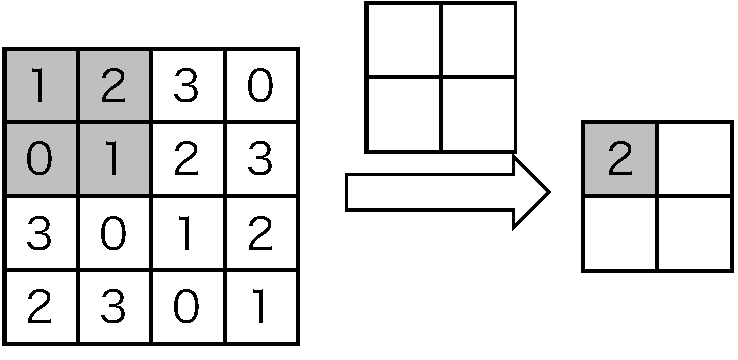
\includegraphics[width=\linewidth]{figure/chapter2/pooling_ex1}
		\subcaption{}
		\label{fig:pooling_ex1}
	\end{minipage}
	\hspace{10truemm}
	\begin{minipage}[b]{0.4\columnwidth}
		\centering
		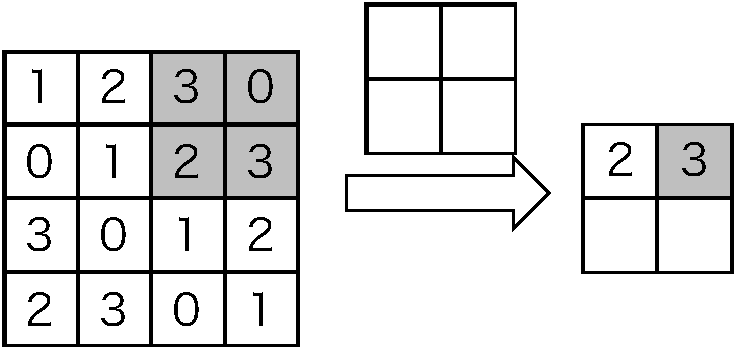
\includegraphics[width=\linewidth]{figure/chapter2/pooling_ex2}
		\subcaption{}
		\label{fig:pooling_ex2}
	\end{minipage}
	\begin{minipage}[b]{0.4\columnwidth}
		\centering
		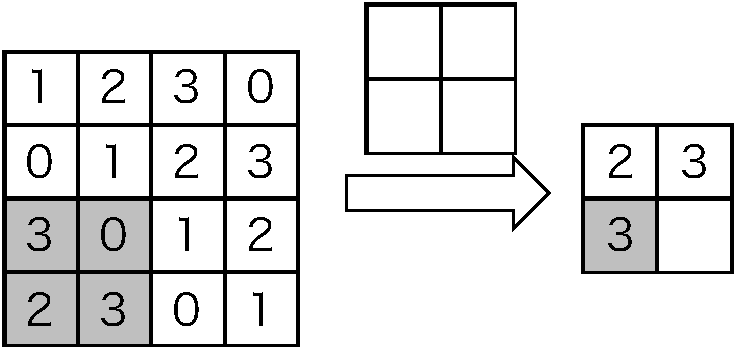
\includegraphics[width=\linewidth]{figure/chapter2/pooling_ex3}
		\subcaption{}
		\label{fig:pooling_ex3}
	\end{minipage}
	\hspace{10truemm}
	\begin{minipage}[b]{0.4\columnwidth}
		\centering
		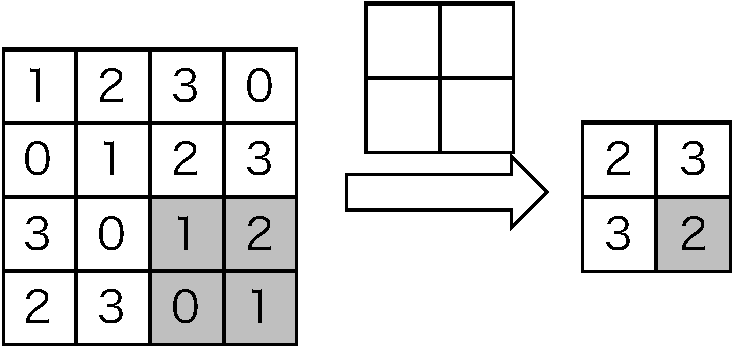
\includegraphics[width=\linewidth]{figure/chapter2/pooling_ex4}
		\subcaption{}
		\label{fig:pooling_ex4}
	\end{minipage}
	\caption{Operation process of max pooling}
	\label{fig:maxpooling}
\end{figure}

プーリング層では画像のサイズを小さくして(コンピュータの)計算コストを減らし,微小な変化に対してロバストになる.

この畳み込みとプーリングを繰り返して,入力からフィルターの数だけ特徴を抽出し,この抽出した特徴マップをFC層へ繋げて識別を行う手法がCNNである.


\section{推論と学習}
ニューラルネットワークでは推論フェーズと学習フェーズに分かれている.\ref{sec:NeuralNetwork}節は全て推論フェーズの話であり,順伝播ニューラルネットと呼ばれる.

学習フェーズでは,逆伝播ニューラルネットを用いる.逆伝播とは誤差逆伝播法(Backpropergation)\cite{Backprop}から由来している.真値からの誤差を表す損失関数(loss function)を用いて,パラメータの微分値を更新に用いる.損失関数はコスト関数,目的関数とも呼ばれる.この微分値を効率よく計算するアルゴリズムが誤差逆伝播法である.

損失関数は解く問題の目的に合わせて選ぶ必要がある.回帰問題では平均二乗和誤差(mean squared error: MSE)が用いられる.
\begin{align}\label{eq:mse}
	L_{\mathrm{MSE}} = \dfrac{1}{2} \sum_{k} (y_k - t_k)^2
\end{align}
また,クラス分け問題では交差エントロピー誤差(cross entropy error)が用いられる.
\begin{align}\label{eq:crossentropy}
	L_{\mathrm{cross}} = - \sum_k t_k \ln {y_k}
\end{align}
ここで,$y$は予測ラベルで,$t$は教師ラベルである.

\subsection{最適化手法}
損失関数を用いてパラメータを更新するが,更新手法にはいくつか方法があるため,ここでは本研究で使用した最適化手法について述べる.

\subsection*{SGD}
SGDは日本語で確率的勾配降下法(Stochastic gradient descent)と呼ばれる手法で,最も単純な最適化手法である.画像認識の分野では多く使われている.

SGDでは以下の式\eq {SGD}でパラメータを更新する.
\begin{align}\label{eq:SGD}
	\bm{W} \leftarrow \bm{W} - \eta \pdif{L}{\bm{W}} 
\end{align}
ここで,$\bm{W}$は更新する重みパラメータ,$\pdif{L}{\bm{W}}$は$\bm{W}$に関する損失関数の勾配である.また$\eta$は学習率と呼ばれ,実際には0.01や0.001といった値を前もって決めて使用する.SGDはパラメータの勾配を利用して,勾配方向にパラメータを更新するステップを繰り返して,徐々に最適なパラメータへと近づける手法である.

\subsection*{Adam}
Adam\cite{Adam}はadaptive moment estimationの略で,勾配の値の1乗和と2乗和の両方をパラメータ更新に用いる手法である.以下の式\eq{adam}でパラメータを更新する.

\begin{align}\label{eq:adam}
	\bm{m} & \leftarrow \beta_1 \bm{m} + (1 - \beta_1) \pdif{L}{\bm{W}} \\
	\bm{v} & \leftarrow \beta_2 \bm{v} + (1 - \beta_2) \left( \pdif{L}{\bm{W}} \right) ^2 \\
	\bm{W} & \leftarrow \bm{W} - \eta \dfrac{\hat{\bm{m}}}{\sqrt{\hat{\bm{v}}} + \epsilon} 
\end{align}

$m_t$と$v_t$はそれぞれ、勾配の一次モーメント(平均値)と二次モーメント(分散した平方偏差)の概算値である.$\eta$,$\beta_1$,$\beta_2$はそれぞれ学習パラメータである.
また,$\hat{m}_t$,$\hat{v}_t$はそれぞれ移動指数平均を用いた際に生じるバイアス(大きさを変えてしまっていることなど)を打ち消すために正則化しており,\eq {adamhat}で表される.

\begin{align}\label{eq:adamhat}
	\hat{\bm{m}} & = \dfrac{\bm{m}}{1 - \beta_1} \\
	\hat{\bm{v}} & = \dfrac{\bm{v}}{1 - \beta_2}
\end{align}

学習パラメータはそれぞれ$\eta = 0.001$,$\beta_1 = 0.9$,$\beta_2 = 0.999$,$\epsilon = 10^{-8}$が最適だと言われている\cite{Adam}.

\subsection{学習のテクニック}
ディープラーニングでは過学習(overfitting)と呼ばれる問題が多く起こる.過学習とは,訓練データに対してのみ適応し過ぎてしまい,訓練データに含まれないテストデータには精度が出ない状態を指す.過学習は,大量にパラメータを持つ表現力の高いモデルであることや,訓練データが少ないことなどが原因で起こる.ここでは過学習を抑制するテクニックを述べる.

\subsection*{Dropout}
Dropout\cite{Dropout}は,ネットワークのノードをランダムに消去しながら学習する手法である.訓練時に隠れ層のノードを毎回ランダムに選択し,そのノードの出力を0にする.そしてテスト時には全てのノードを活性化させ,信号を伝達させる.

Dropoutは,学習時にノードをランダムに消去することで,毎回異なるモデルを学習していると解釈でき,アンサンブル学習と同じ効果を擬似的に1つのネットワークで実現していると考えられる.アンサンブル学習とは,弱識別器を複数合わせて1つの強力な識別器とする手法で,現在でも有効な手法として用いられている.

\subsection*{Batch Normalization}
Batch Normalization\cite{BatchNorm}は,ネットワークにおける各層での活性化後の出力(アクティベーション)の分布を,適度な広がりを持つように調整する手法である.Batch Normalizationでは学習を行う際のミニバッチを単位として,ミニバッチごとに正規化を行う(\eq {BatchNorm}).
\begin{align}\label{eq:BatchNorm}
	\mu_B & = \dfrac{1}{m}\sum_{i=1}^m x_i \\
	\sigma_B^2 & = \dfrac{1}{m}\sum_{i=1}^m (x_i - \mu_B) \\
	\hat{x_i} & \leftarrow \dfrac{x_i - \mu_B}{\sqrt{\sigma_B^2 + \epsilon}}
\end{align}
ミニバッチとして$B = \{x_1, x_2, \cdots, x_m\}$という$m$個の入力データの集合に対して,平均$\mu_B$,分散$\sigma_B^2$を求め,入力データを平均0分散1となるように正規化を行う.$\epsilon$は0で除算されることを防ぐもので,極小の値を用いる.

Batch Normalizationを用いると,学習を速く進行させることができる,初期値にそれほど依存しない,過学習を抑制できるといった効果が期待できる.


\section{画像認識と深層学習}
Deep LearningとはDeep Neural Network(DNN)を指すことが多い.この"Deep"とは,ニューラルネットワークの層が深いことに由来している.

\fig {ImageNet}に画像認識タスクの精度の近年の推移を示す.これはImageNet Large Scale Visual Recognition Challenge (ILSVRC)と呼ばれる世界的な画像認識のコンペティションである(2010年から始まった).カテゴリ数は1000クラスで,画像枚数は120万枚の訓練データと15万枚のテストデータが用意されている.
\begin{figure}[H]
	\centering
	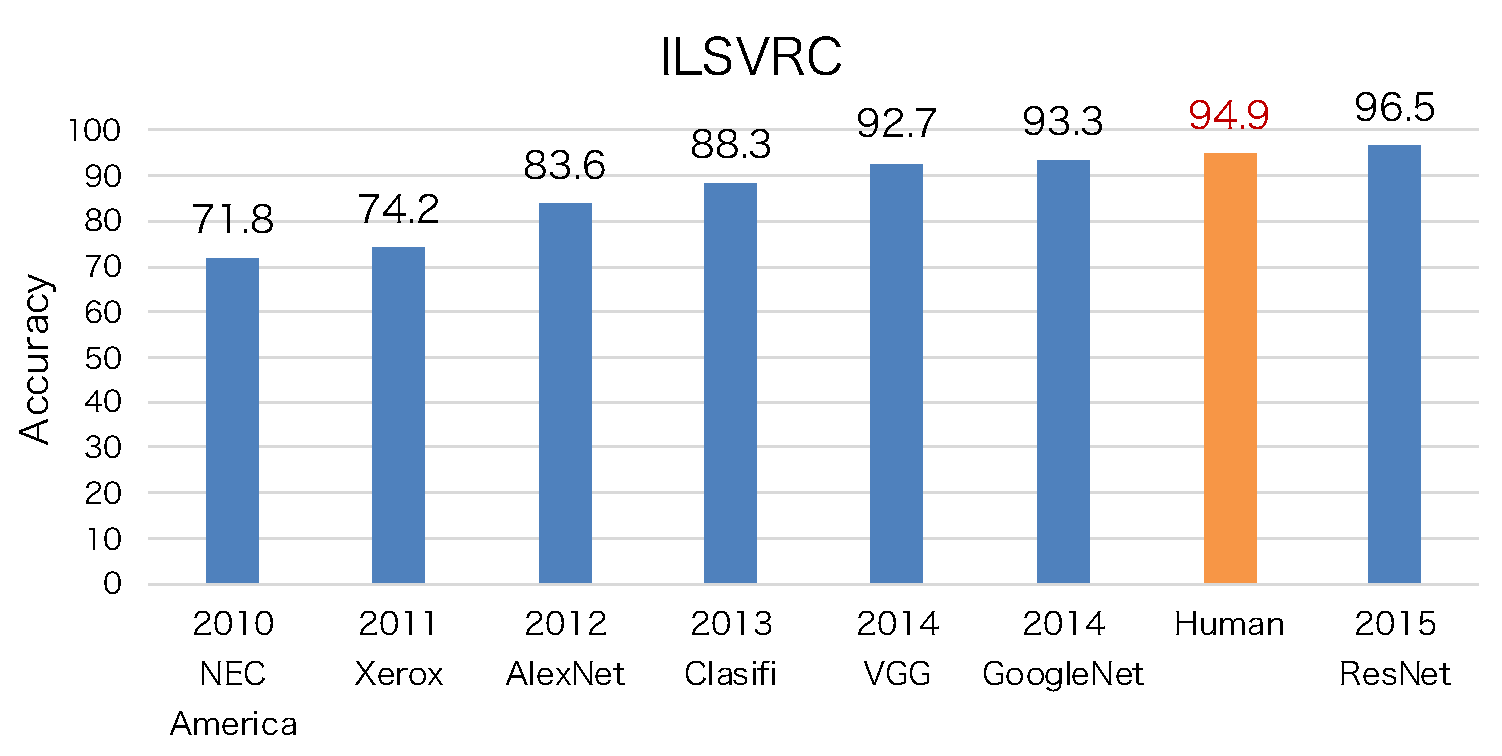
\includegraphics[width=0.7\linewidth]{figure/chapter2/ILSVRC}
	\caption{Transition of accuracy of image recognition on ILSVRC}
	\label{fig:ImageNet}
\end{figure}
2011年と2012年は約10\%もの大差でAlexNet\cite{AlexNet}が優勝している.これがディープラーニングの始まりである.AlexNetは5つの畳み込み層と3つの全結合層を持っている.2014年にはVGGNet\cite{VGGNet}やGoogLeNet\cite{GoogLeNet}が9割の精度を超えた.VGGNetはAlexNet(8層)よりさらに深い構造(19層)であり,GoogLeNetは22層もある.そして2015年にはResNet\cite{ResNet}が人間の精度をも超える認識精度を達成した.ResNetはGoogLeNetよりもさらに深く152層もある.CNNを複数回かけて検出を行う場合,CNNの浅い側では空間分解能はあるが抽象的な情報が少ない.深い側では意味論的な情報は取得できる(ポーズ,変形など)が空間分解能が小さいため幾何学的な情報が失われる.

アーキテクチャの進化の方向は大きく3つある.1つ目は層を深くすることである.2つ目はFC層の使用を避ける,またはInceptionモジュールの使用することである.これにより学習するパラメータ数を削減することができる.3つ目はResNetなどのショートカット接続の利用や,事前学習・転移学習を行うことである.これによって学習効率を向上させ,最終的にモデルの精度向上へと繋がる.ここで,事前学習のデータセットと適用データとの間には類似性があると良い.

画像処理におけるディープラーニングでは大きく3つのタスクがあり,それぞれ,クラス分類,物体検出,セグメンテーションである.以下に詳細を述べる.

\subsection*{クラス分類}
クラス分類は画像に写っている物体が「dog」「airplane」「bird toy」など事前に定義されたラベルのどれが適切かを識別するタスクである.この識別は,事前に定義されたラベルの特徴べクトルと入力画像の特徴べクトルの距離計算を行い,距離値が小さければ同一,そうでなければ否と判定する.指紋照合,顔照合,人物照合では,本人と他人を判定するタスクとなる.深層学習では,同一人物のペア画像間の距離値が小さく,他人の画像との距離値が大きくなるような損失関数を設計し,ネットワークを構築することで人物照合問題を解いている.

\subsection*{物体検出}
物体検出とはBounding Boxで物体の位置とその物体の種類を特定する方法である.歴史的には幾何的情報,手動特徴量,そしてそのカスケードを利用していた.その後,HOG\cite{HOG}やSIFT\cite{SIFT}など局所特徴量を抽出する方法を設計するようになったが,これは深い専門知識を必要とした.また広い範囲でオブジェクトを正確に検出する方法は,メモリ容量と処理時間に課題がある.現在はDeep Neural Networkが主流となり,データのみから抽象的な特徴量を複数得ることができる.

物体検出で主流であるのはFaster R-CNNである\cite{faster_R-CNN}.

Faster R-CNNよりも高速に検出を行えるようにしたのが,SSD\cite{SSD}とYOLO\cite{YOLOv3}である(\fig {SSD}).クラス分けの場合は数1000のカテゴリを学習してTop Error Rateが2\%以下と人間よりも認識精度が高いが,物体検出においては,現状ではカテゴリが数100程度くらいまででも認識精度が人間よりも低くなってしまう.また物体検出は精度を上げるために処理に時間がかかることが多いため,リアルタイムに物体検出を行う時は,速度と精度のトレードオフが生じてしまう.

\begin{figure}[H]
	\centering
	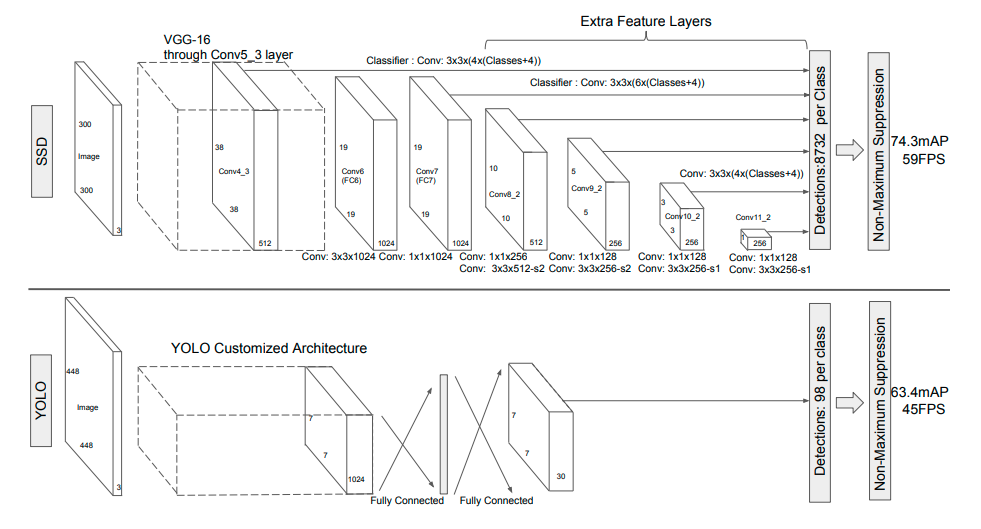
\includegraphics[width=0.7\linewidth]{figure/chapter2/yolo_ssd.png}
	\caption{Network Architecture of SSD and YOLO\cite{SSD}}
	\label{fig:SSD}
\end{figure}

\subsection*{セグメンテーション}
セグメンテーションにはセマンティックセグメンテーションとインスタンスセグメンテーションの2つがある.

セマンティックセグメンテーションとは,画像を画素レベルで認識することである.画像内の各画素をオブジェクトクラスに割り当てる手法である.セマンティックセグメンテーションの手法についてディープラーニング以前では,Texton Forests\cite{shotton2008semantic}や,Random Forests\cite{kontschieder2011structured}に基づいた分類を行っていたが,物体検出と同様にCNNが登場してからは,高精度なセグメンテーションが実現するようになった.CNNを使ったセグメンテーションの手法で一般的に使われるようになったものがUnetである\cite{Unet}.このUnetは文字通りUの形をしたネットワークであることが特徴で,2つのアーキテクチャーからできている(\fig {Unet}).1つ目がエンコーダーのアーキテクチャーでCNNとプーリングで特徴を抽出しながら次元を削減していき,2つ目のデコーダーのアーキテクチャーで画像をセグメンテーションの結果になるように復元する.ここで問題になることが,プーリングをすることで位置情報を消してしまっているので,この位置情報を利用して画像を復元するためには,エンコーダーとデコーダーで画像サイズが同じところ同士をショートカットで接続することがUnet構造の優れている点である.

\begin{figure}[H]
	\centering
	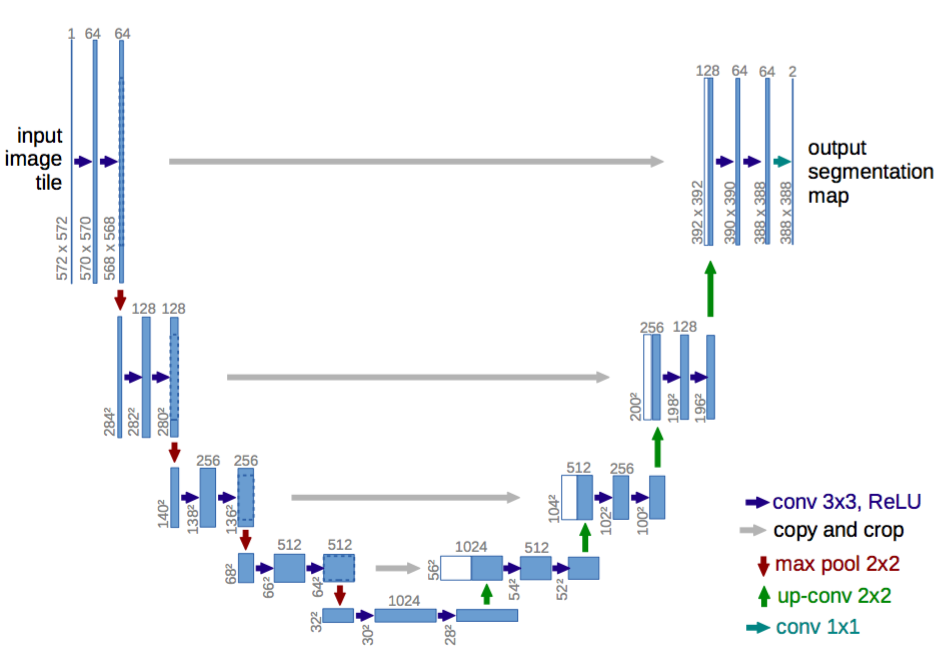
\includegraphics[width=0.7\linewidth]{figure/chapter2/unet.png}
	\caption{Artchitecture of Unet\cite{Unet}}
	\label{fig:Unet}
\end{figure}

インスタンスセグメンテーションとは,同じクラスの物体も別として認識することである.まず,入力画像に対して物体検出を行い,検出したBounding Box内でセグメンテーションを行う.すなわち,インスタンスセグメンテーションは物体検出とセマンティックセグメンテーションのハイブリッドと言える.インスタンスセグメンテーションでよく使われる手法はMask R-CNNである\cite{Mask_R-CNN}.




\section{強化学習}\label{sec:強化学習}
% 上の話は教師あり学習で,ここからは強化学習という分野である.
今まで述べてきたことは全て教師あり学習と呼ばれる手法であり,機械学習の1種である.ここからは強化学習という機械学習について述べる.

\subsection{マルコフ決定過程}
\fig {RLframework}に強化学習の概念図を示す.強化学習は,エージェントと呼ばれるプレーヤーが,与えられた環境と相互作用し,探索と知識の利用を行って目標を達成する方法を求める.強化学習は教師あり学習に似ているが,教師による明確な「答え」は提示されない.代わりに「行動の選択肢」と「報酬」が提示される.ここで,強化学習においての報酬は「各行動」に対してではなく,「連続した行動の結果」に対して与えられる.この報酬を最大化することが強化学習の目的である.
\begin{figure}
    \centering
    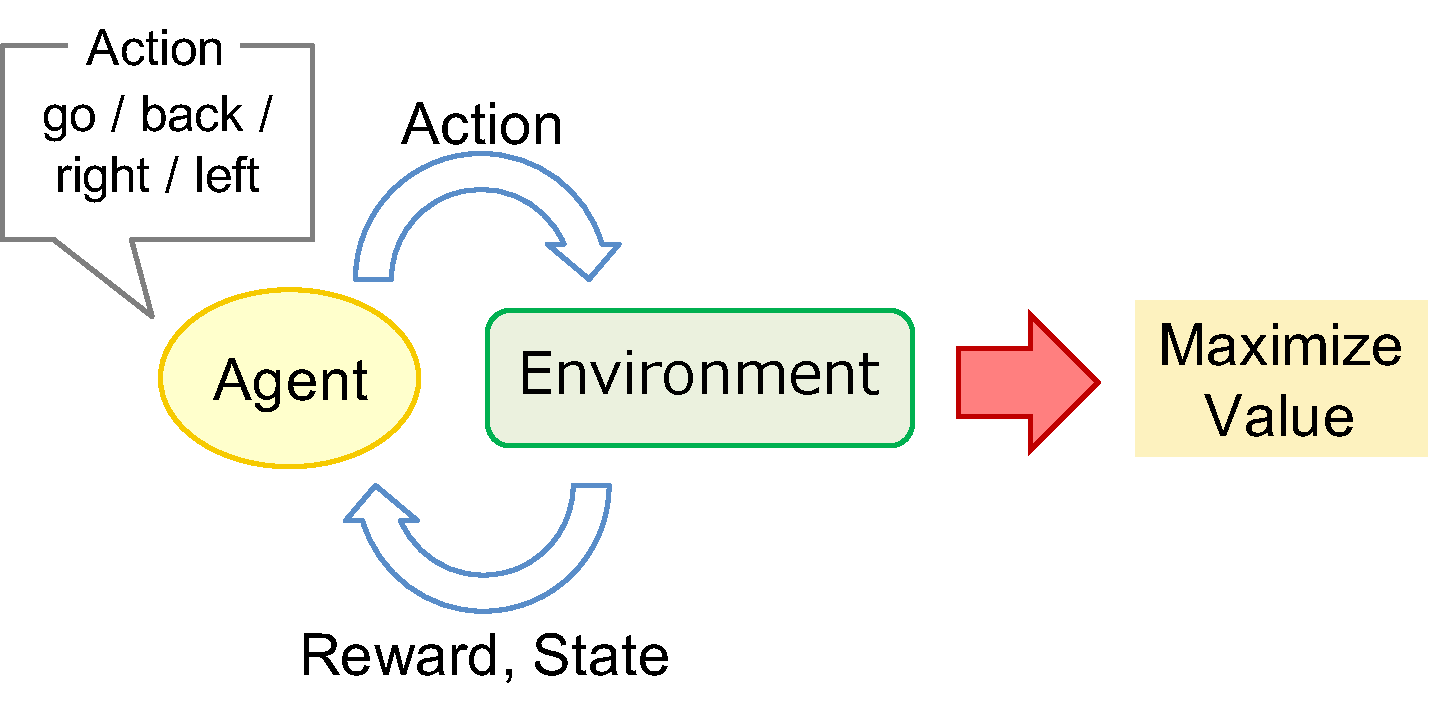
\includegraphics[width=0.7\linewidth]{figure/chapter2/RL_framework}
    \caption{Framework of Reinforcement learning}
    \label{fig:RLframework}
\end{figure}
この\fig {RLframework}を表す数理モデルとして,マルコフ決定過程(Markov Decision Process: MDP)がある.MDPは時刻$t$における状態を$s_t$,行動を$a_t$,報酬を$r_t$,状態$s_t$における行動を返す方策$\pi(a_t|s_t)$,次の状態$s_{t+1}$へ移る状態遷移確率$P(s_{t+1}|s_t, a_t)$によって記述される確率過程である.マルコフというのはマルコフ性という意味で,次の行動$s_{t+1}$には現在の状態$s_t$しか関与しないという性質を表している.1回の報酬を指標にに最適な行動を求めてはすぐに局所解に落ち着いてしまい,後に来る大きな報酬を得ることができないため,よい指標にはならない.そこで,ある期間で得られた累積の報酬(収益)$R_t$を導入する.
\begin{align}\label{eq:reward}
    R_t & = \sum _{\tau=0} ^{\infty} \gamma ^\tau r_{t+1+\tau} \\
        & = r_{t+1} + \gamma r_{t+2} + \gamma ^2 r_{t+3} + \cdots
\end{align}
と表され,これを割引報酬和(discounted total reward)と呼ぶ.ここで$\gamma(0<\gamma<1)$は割引率と呼び,未来の報酬をどの程度割り引くかを決めている.概ね1に近い値を用いる.この収益は,機関の中で報酬の和を取るため,ある行動が期間内における報酬の獲得に結び付いていた場合には,それがずっと後のことであっても,指標に反映することができる.

しかし収益は,区間の開始時点での状態に依存して,相互作用の内容が確率的に決定されるため,収益も確率的に変動してしまう.そのため,状態$s$と行動$a$を条件として収益の期待値を取り,これを行動価値(action value)と呼ぶ.行動価値関数$Q(s,a)$は,ある状態から方策$\pi$に従って行動を決定したときに得られる収益の期待値であるから,

\begin{align}\label{eq:Qfunction}
  Q^{\pi}(s_t, a_t) & = \mathbb{E}\bigl[ \bigl. R_{t+1} \bigr| s_t, a_t\bigr] \\
    & = \underset{s_{t+1}, a_{t+1} }{\mathbb{E}}\bigl[ \bigl. r_t + \gamma Q^{\pi}(s_{t+1}, a_{t+1}) \bigr| s_t, a_t \bigr]
\end{align}
で表される.これを指標として,最適な方策$\pi ^*$に基づく最適行動価値関数$Q^*$を求める.

最適価値関数を求める方法として,Temporal-Difference Learning(TD学習)が用いられる.TD学習は,環境のモデルを使わず経験的に学習を行い,最終結果を待たずに評価を途中で更新する.TD学習は次のステップを待ち価値関数を更新する.
\begin{align}\label{eq:TD}
Q(s_t, a_t) \leftarrow & Q(s_t, a_t) + \alpha (r_{t+1} + \gamma Q(s_{t+1}, a_{t+1}) - Q(s_t, a_t) )
\end{align}
$\alpha(0<\alpha<1)$は学習率である.ここで,$r_{t+1} + \gamma Q(s_{t+1}, a_{t+1}) - Q(s_t, a_t)$をTD誤差と呼び,収束からの離れ具合を示す.学習が収束したとすればTD誤差が0になり,その収束値が最適価値関数となる.

\subsection{Q-Learning\cite{QLearning}}
Q学習では,TD誤差に基づいて次のように価値関数$Q$を更新する.
\begin{align}\label{eq:Qupdate}
    Q(s,a) \leftarrow & Q(s,a) + \alpha (r + \gamma\underset{a'}{\max}{Q(s',a')} - Q(s,a))
\end{align}
更新式で実際に採用した行動$a'$を使っていない(方策に関わらず価値関数の最大値を与える行動を使っている)ことが特徴である.ここで,方策$\pi$としては,まずはランダムに行動することで状態と行動のセット$(s,a)$を蓄積していき,その中で行動価値関数が最大となるような行動を取る.これを$\epsilon$-greedy方策と呼ぶ.確率$\epsilon$でランダムに行動することで,局所解に陥らずに最大値へ収束することができる.

端的に言えば,「どの状態で、どう行動したら、どういう報酬が得られるのか」を明らかすることがQ-Learningである.実際はこの報酬の見込みの表形式で表し,これをQ-Tableと呼ぶ.

Q-LearningはQ-Tableが求まれば良いが,環境から得られる状態の次元や行動の次元が大きいと求められない場合がある.そのため,Q-Learningを設計する場合は,環境から特徴を取り出し低次元にする必要がある.また,行動も連続的な行動ではなく,離散的な行動選択に絞る必要がある.


\subsection{強化学習のロボット制御への応用}
Guらは人間の手を介さずドアを開ける動作を初めて成功させた\cite{Gu2017}(\fig {Gu}).ここでは,Q-LearningをベースとしたNormalized Advantage Function(NAF)という手法を用いている.観測する状態として,7つの間接角度とその時間微分,ハンドエフェクタ・手・ドアのそれぞれの位置,手・ドアのそれぞれの角度の計25次元を入力し,Actionは連続値で出力する.シミュレーション上で4機で非同期分散学習させた後,実世界では最大2機で非同期分散学習を行った.実世界では成功率100\%になるまでに1機では4時間,2機では2.5時間という短い時間で達成した.シミュレーションから実世界への転移は難しいことが多く,Guらは成功判定を緩めることで解決した.
\begin{figure}
    \centering
    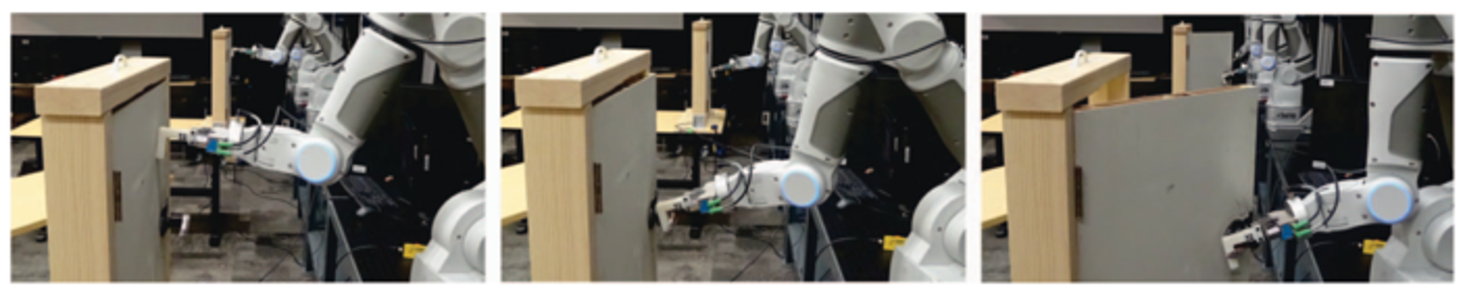
\includegraphics[width=\linewidth]{figure/chapter2/Gu}
    \caption{Two robots learning to open doors using asynchronous NAF. The final policy learned with two workers could achieve a 100\% success rate on the task across 20 consecutive trials\cite{Gu2017}.}
    \label{fig:Gu}
\end{figure}

Levineらは初めてvisionベースでグラスピングタスクを成功させた\cite{Levine2017}(\fig {Levine}).この手法は厳密にはQ-Learningではないが,Q-Learningとも解釈できると言っている.入力としてRGBの画像とモーターのコマンドを入れ,出力として把持可能性を確率で返す.最大14台のロボットで非同期分散学習を行い,800,000回以上の試行を行った.
\begin{figure}
    \centering
    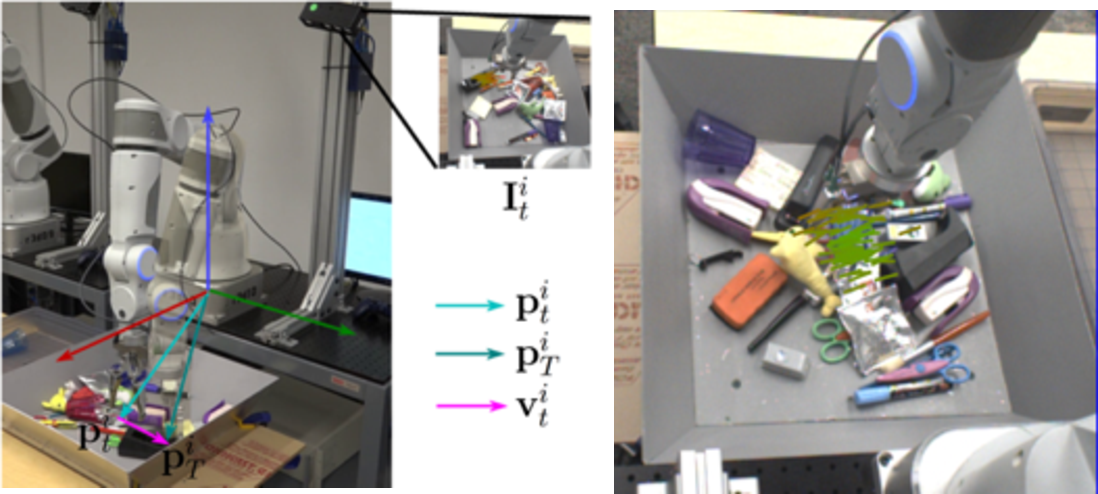
\includegraphics[width=\linewidth]{figure/chapter2/Levine_grasp}
    \caption{Col- ors indicate their probabilities of success: green is 1.0 and red is 0.0\cite{Levine2017}.}
    \label{fig:Levine}
\end{figure}

またDmitryらは,Q-Learningを改良したQT-optという手法を提案した\cite{Dmitry2018}(\fig {Dmitry}).これはより汎用性の高いタスクをロボットに学習させることを目的として,1000種類以上の物体を把持できるような学習を行った.QT-Optを実行すると、より多くのオフラインデータが蓄積され,より良いデータを収集できるように,より良いモデルを訓練できるようになる.このアプローチを使い,ロボットで物を掴む事を学習させるために7つの実世界のロボットを使用し,4ヶ月間にわたって合計800時間学習させた.学習を早めるために,最初は人間が手動で設計した15~30\%程度の成功率のポリシーを使用して開始した.状態としてRGBのカメラ画像を取得し,行動として腕とグリッパの移動方法を返す.報酬は成功したら+1,失敗したら0としている.また,失敗した時の報酬を-0.05とすると学習を早めることができる.シンプルな仮定ではあるが,QT-optは目標物体を掴むために周りの邪魔な物体を弾いたり,掴みやすいように物体を倒したりすることを学習した.また,従来の手法より少ない学習データで高い成功率を達成した.

\begin{figure}
    \centering
    \includegraphics[width=\linewidth]{figure/chapter2/Dmitry}
    \caption{Pregrasp manipulation (a, b), grasp readjustment (c, d), grasping dynamic objects and recovery from perturba- tions (e, f), and grasping in clutter (g, h)\cite{Dmitry2018}.Video: \url{https://sites.google.com/view/qtopt}}
    \label{fig:Dmitry}
\end{figure}


OpenAIチームはvisionベースで自由度が26もある手を模したロボットでサイコロを任意の向きに変える複雑な動作を達成した\cite{OpenAI2018}(\fig {OpenAI}).今回は方策を直接学習するProximal Policy Optimiztion(PPO)と呼ばれる手法を用いている.状態として3つのカメラからのRGB画像を与え,行動として接続部の角度を返す.報酬として成功したら+5,失敗したら-20,途中の報酬は現在とゴールの回転角度の差分を与えた.シミュレーション上で環境にノイズを加えて学習することで,実世界においても性能を発揮できるような学習を行ったことがポイントである.
\begin{figure}
    \centering
    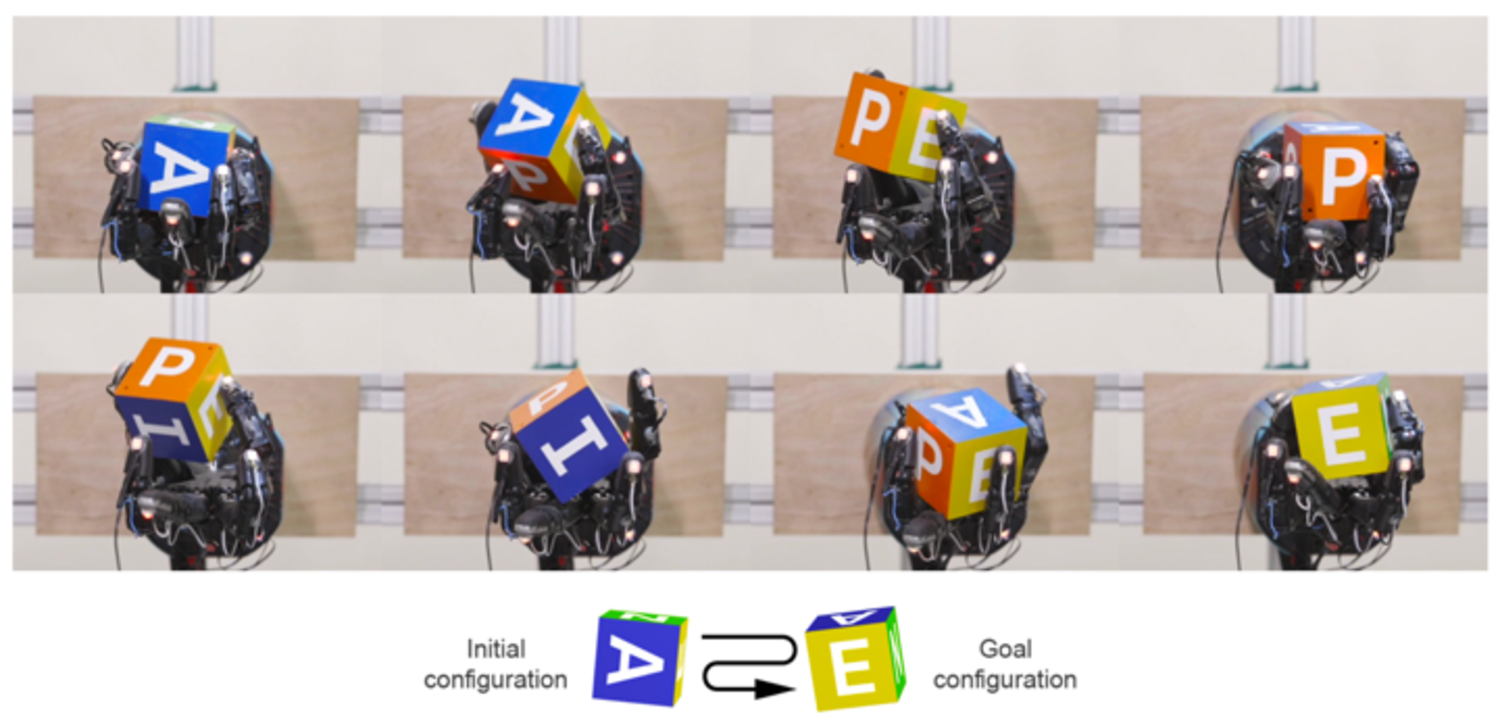
\includegraphics[width=\linewidth]{figure/chapter2/openAI_cube}
    \caption{A five-fingered humanoid hand trained with reinforcement learning manipulating a block from an initial configuration to a goal configuration using vision for sensing\cite{OpenAI2018}.Video:\url{https://blog.openai.com/learning-dexterity/}}
    \label{fig:OpenAI}
\end{figure}
 % 原理
\chapter{試作1号機:スマートフォン搭載ハンドの開発}
\newpage

%ここに3章の概要(本章での背景,目的(動機),章内の節構成について言及してやると,何を述べているのか理解しやすい.
%(モバイル)ロボットハンド作製を通じ,実用化のための課題点を整理する.
\section{要求仕様}
%1章で修論全体もしくは一般的な夢物語を述べて,3章ではその達成のための布石として,必要なスペックを述べる必要がある.いきなり節から始めるのであれば,ここにその内容を再度記載しておく方が親切な気がする.

1号機では本体の基本デザイン・自律動作・携帯性に重点をおいて設計する.

ハードウェアとして自律移動が可能で物体を把持でき,また小型で携帯可能な重量が要求される.そのため,環境を認識できるセンサ,対象物に接近するためのアクチュエータ,把持を行うためのアクチュエータ,これらを制御するコンピュータが必要である.

ソフトウェアとして,センサ情報をEdgeで計算しアクチュエータ制御を行うことが要求される.また持ち運ぶため環境にロバストな制御方式であることが必要である.ただし,衝突リスク等を考慮するとアクチュエータの制御は高速に行う必要はなく,数ミリ秒毎に制御する高速動作は求められない.


\section{機構設計・機体デザイン}
環境を把握するセンサとして,簡便でかつ情報量の多いカメラを採用した.また自律移動には車輪を採用し,後輪駆動の3輪車とした.車輪の駆動にはDCモーターを用いた.把持動作にはサーボモータを使用し,1軸の握る動作を実装した.

上記の画像取得,認識,処理,アクチュエータ制御をすべてスマートフォンで実現を試みた.ロボットハンドにはスマートフォンを搭載し,スマートフォンのフロントカメラから環境を認識させた.アクチュエータの制御にはワンチップコンピュータを使用し,スマートフォンとシリアル通信を行うことで各アクチュエータをそれぞれ制御した.

これらを考慮して\fig{1号機CAD}に示すようなフレームを3DCAD(123D Design Autodesk社を使用)で設計した.また,ロボットハンドの向きは\fig{1号機CAD}に示す,ソフトウェアでの画像(配列)の向きと同様の定義とした.

\begin{figure}[H]
    \centering
    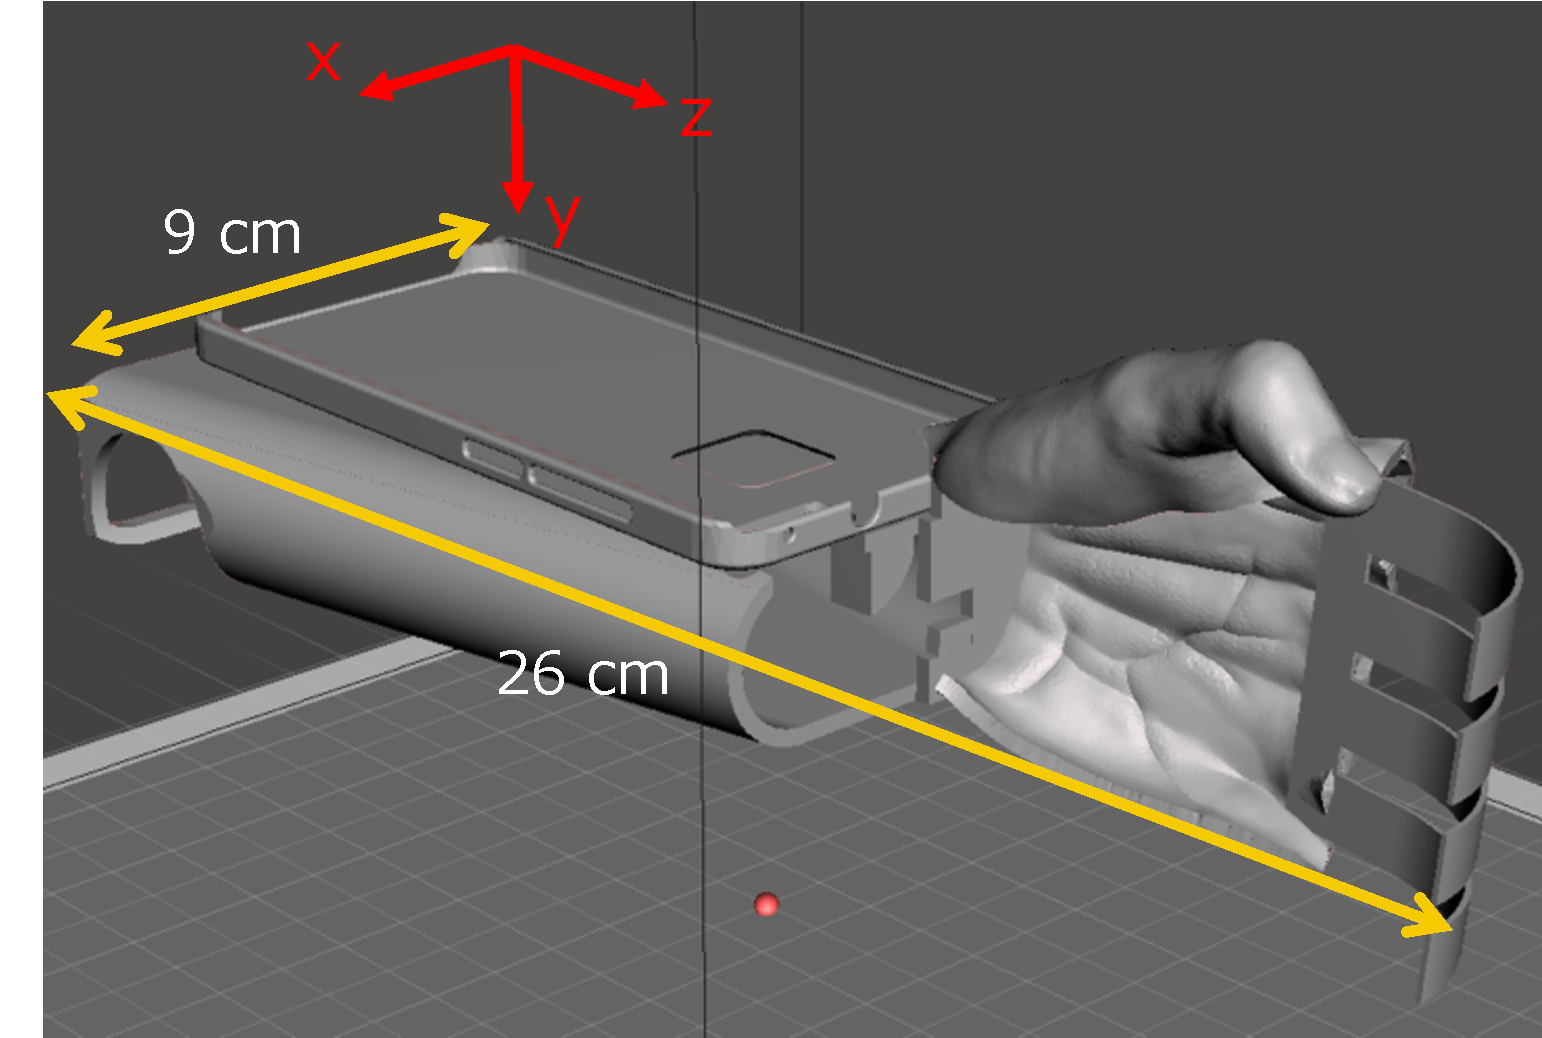
\includegraphics[width=\linewidth]{figure/chapter3/1号機CAD}
    \caption{3DCAD image of prototype No.1}
    \label{fig:1号機CAD}
\end{figure}


\section{制御アルゴリズム}
自律移動のアルゴリズムは強化学習で行った.強化学習は環境に対してロバストであるため,実生活において有用だと考えた.強化学習の最適化としてはQ-Learningを用いて学習を行い,方策として$\epsilon$-greedy方策を使用した.

\fig{1号機制御図}に1号機の制御系ブロック図を示す.ロボットハンドの接近動作のフローを述べる.
まず,フロントカメラから480x640 pixelの画像を取得する.取得した画像をHSV空間に変換し,赤色だけを抽出しターゲットのマスク画像を得る.マスク画像からターゲットの面積(ピクセル数)と画像における重心を求め,面積を画像サイズで規格化した.この面積値と前フレームでの面積値との差分の2次元を状態として与えた.行動として前進,後退,右旋回,左旋回の4次元を与えた.報酬としてタスクが成功したら+1,1episode以内で成功できなかったら-1,その他では0とした.episodeの終了判定に面積値と重心座標を用いて,面積が40以上で最接近とし,また重心座標がロボットの中心座標から10pixel以内であれば正面に来たと判定した.接近が完了したらサーボモータを動かして対象物を握るようルールベース化した.

\begin{figure}[H]
    \centering
    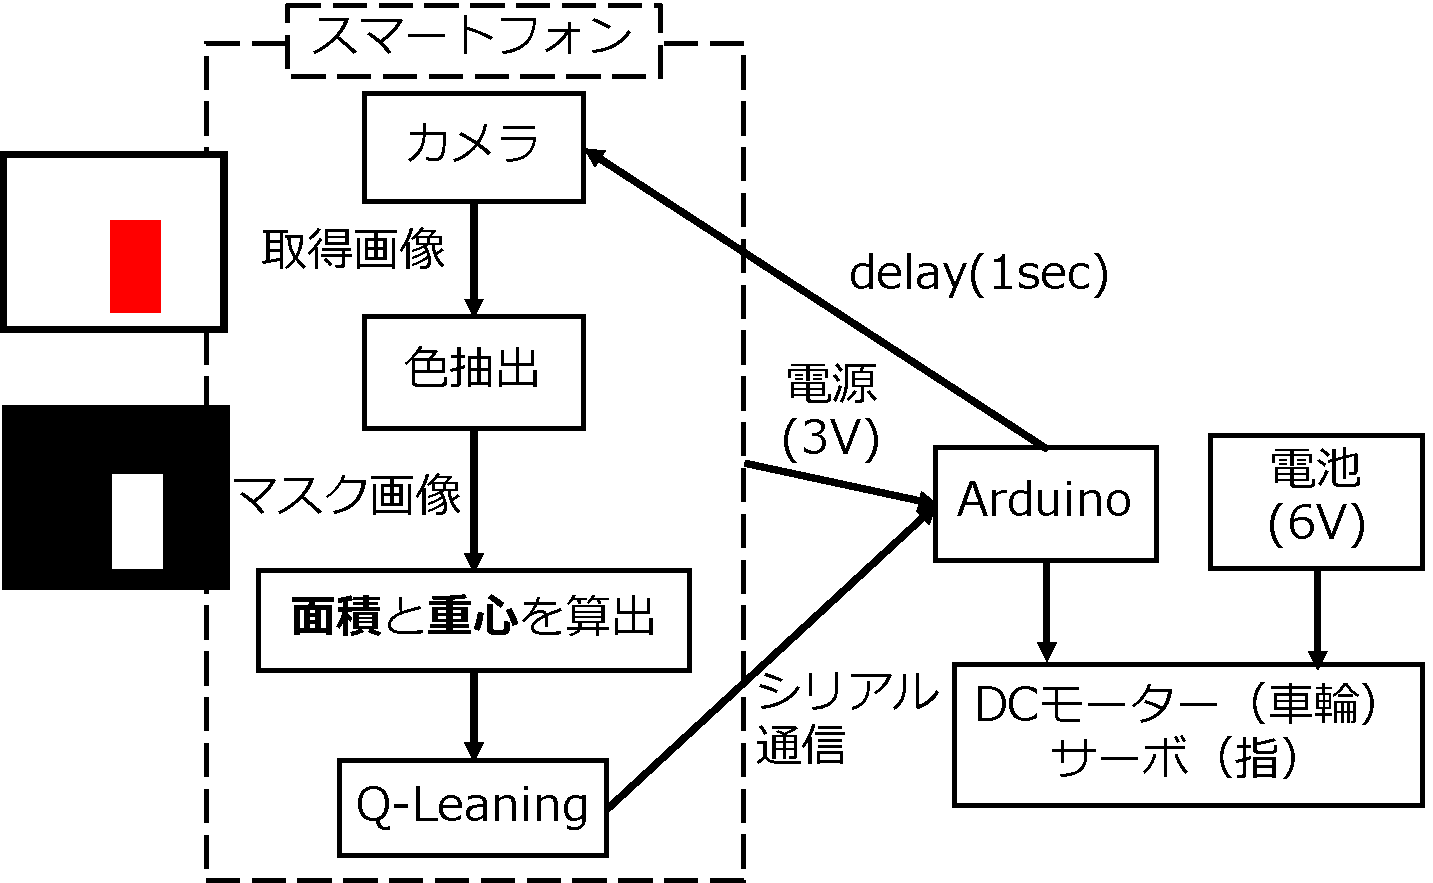
\includegraphics[width=0.7\linewidth]{figure/chapter3/1号機制御図-2}
    \caption{Block diagram of Prototype No.1}
    \label{fig:1号機制御図}
\end{figure}


\section{実機作製}
1号機作製にあたって使用した部品を\tab{1号機部品}まとめた.

\begin{table}[H]
    \centering
    \caption{Components of prototype No.1}
    \begin{tabular}{cc}\toprule
        本体フレーム & PLA(黒) \\
        スマートフォン & HUAWEI P10 lite \\
        DCモーター & \href{http://akizukidenshi.com/catalog/g/gM-12379/}{STLギヤモータ 栄42D長軸型} \\
        サーボモータ & \href{http://akizukidenshi.com/catalog/g/gM-01908/}{GWSサーボ MICRO/2BBMG/FP(フタバ)} \\ 
        タイヤ & \href{https://tamiya.com/japan/products/70194/index.html}{TAMIYA製スパイクタイヤ} \\ 
        コンピュータ & \href{http://akizukidenshi.com/catalog/g/gK-10347/}{ArduinoProMini} + \href{https://www.switch-science.com/catalog/1032/}{FTDI} \\ 
        バッテリー & 単4電池x4本 + 電池パック \\
        \bottomrule
    \end{tabular} 
    \label{tab:1号機部品}
\end{table}

ロボットハンドのフレームは簡便さと軽さを考慮し3Dプリンタ(TITAN GENKEI社)で造形を行った.\fig{1号機外観}に作製したロボットハンドの外観を示す.スマートフォンは腕の上部に装着し着脱ができるようにした.スマートフォンのフロントカメラに鏡を角度45度傾けてで置くことでz軸方向(スマートフォンの上側方向)を捉えることができるようにした.また,腕部分にバッテリーとタイヤ,そしてArduinoを含む回路を収め,上から見るとスマートフォンと手のみが見えるように工夫して組み立てた.1号機の総重量は473.82 gであった.

\begin{figure}
    \centering
    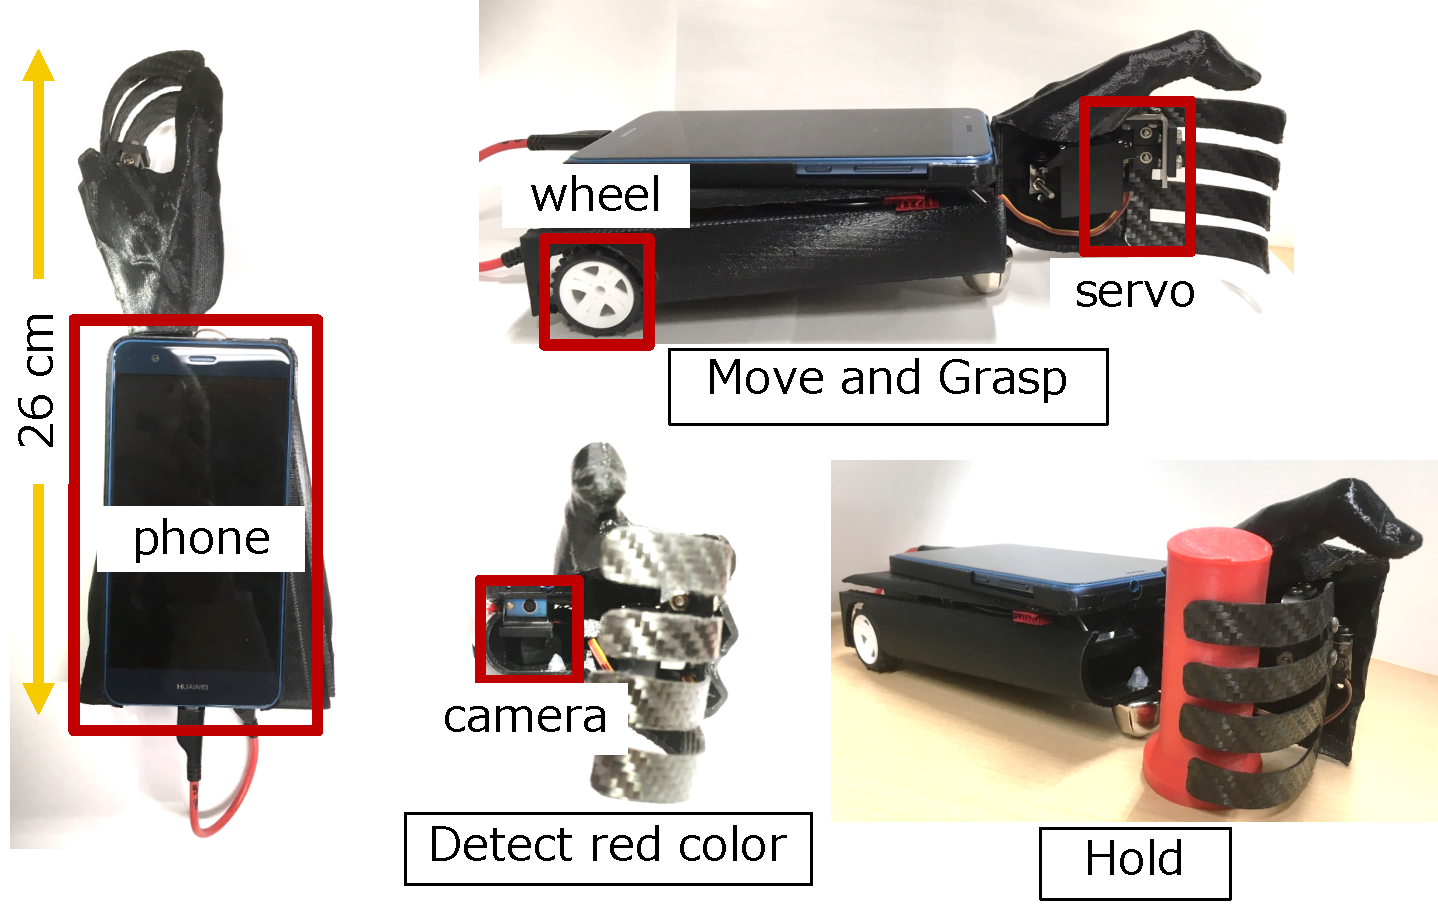
\includegraphics[width=\linewidth]{figure/chapter3/1号機外観}
    \caption{Appearance of prototype No.1 made of 3D printer. Weight is 473.82 g.}
    \label{fig:1号機外観}
\end{figure}


\subsection{学習方法}
1号機の行うタスクとして接近タスクを行った.実機で2日間に渡り約300episodes学習させた.
Q-learningのハイパーパラメータは,割引率は0.99,学習率は0.5,状態は6つの状態に離散化した.


\subsection{結果}
学習の中で成功したepisodeにおけるロボットの挙動を\fig{1号機例}に示す.まず,旋回することであたりを探索する.カメラにターゲットを捉えたらそれに向かって接近し,一定の距離まで近づいたら把持を行う.このような流れで学習が進んでいることが示唆された.

\begin{figure}[H]
    \centering
    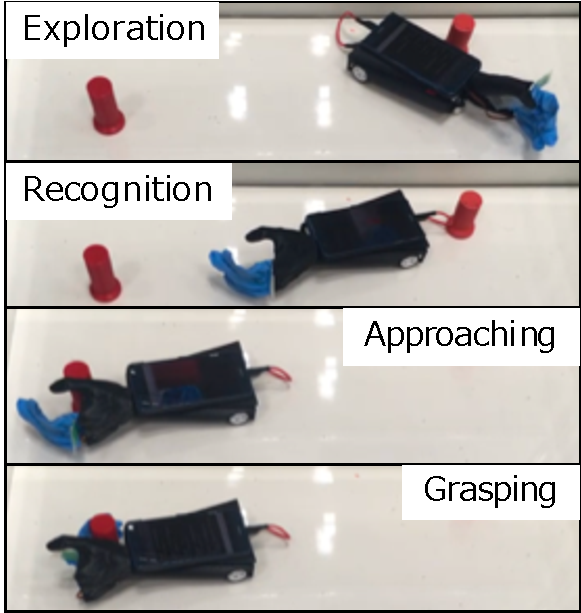
\includegraphics[width=0.7\linewidth]{figure/chapter3/robothand-v1_demo}
    \caption{Demonstration of prototype No.1 at sucess episode.}
    \label{fig:1号機例}
\end{figure}

しかしカメラのフレームレート(frame per second: fps)が低く1fps程度であり,各stepにおける行動が1秒程度持続してしまい,同じ場所を旋回しつづける行動が問題であった.fpsが低い原因として,スマートフォンのカメラにプロテクトがかかっておりビデオが使えず,カメラの単写を使用せざるを得ないことが挙げられる.またスマートフォンの演算能力ではより高次元の状態や行動を入出力とした強化学習は難しいため,"曲がりながら進む"といった前進と旋回の組み合わせができなかった.


\section{物理シミュレーション}
強化学習では学習に多くの時間がかかる.また実機ではバッテリー残量や壁にぶつかった際に位置を人の手で直す必要がある.そこでより学習を進めかつ自動で学習ループを回すために物理シミュレーションを用いた.これにより学習過程を常に記録・参照することもできる.


\subsection{評価手法}
シミュレーション物理エンジンとしてBullet Physics Engineを用いた.実装においてはAPIがPythonで用意されているPyBullet\cite{pybullet}を使用した.\fig{1号機simu}にCADで作製したロボットハンドをシミュレーション環境にレンダリングした画像を示す.

\begin{figure}[H]
    \centering
    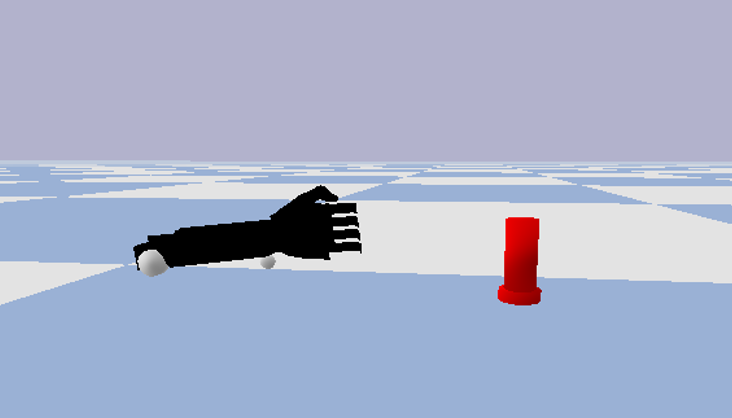
\includegraphics[width=0.7\linewidth]{figure/chapter3/bullet_demo}
    \caption{Environment of bullet physics simulation.}
    \label{fig:1号機simu}
\end{figure}

ターゲットをランダムに配置し,観測状態と報酬を変えて学習がどのように進むかを実験した.タスクとしては接近のみを行い,ルールベース化してある把持は省略した.性能をテストする際,$\epsilon$-greedy方策の探索する確率を0とし,greedy方策でテストする.そして10episodeごとに報酬の総和を計算し,1episodeあたりの報酬として平均をとった.


\subsection{結果}
まず,状態としてカメラから認識できるターゲットの面積値(最大を100に規格化),及びそのフレーム間差分の2次元を与えた.また報酬として,タスクが成功したら+1,1episode以内に成功しなかったら-1,各stepでは0とし,学習を行った(\fig{報酬離散}).Episodeが経過しても報酬に変化がないことから,学習が収束していないことがわかる.この原因としては観測が良くないかまたは報酬設計が悪いかの2つが考えられる.Agentの行動は環境から得られる報酬に依ることを考慮すると,多くのepisode学習を行っても収束しないということは観測状態が良くないと考えられる.また,報酬は連続値で与える方が各episodeごとではなく各stepごとにパラメータ更新が行えるため学習がスムーズに進むので,報酬を連続値に変えた.

次に,状態としてロボットハンドとターゲットとの相対位置$(x,y)$座標の2次元を与えた.また報酬として,ターゲットとの距離を与え,学習を行った(\fig{報酬距離}).\fig{報酬離散}とは挙動が異なり,初めの数10episodeで急激に報酬が増加し,その後横ばいとなっていることがわかる.Episodeを重ねても報酬は飽和しているため,学習が収束していることがわかる.このパラメータでレンダリングして確認してみると,学習が成功していることが分かった.

また,状態としては先ほどと同様に相対位置$(x,y)$座標の2次元を与え,報酬としてターゲットの面積値を与え学習を行った(\fig{報酬面積}).Episodeが進むとなだらかに報酬が増加し,400episode付近から報酬が飽和していることがわかる.このことから学習が収束していると言える.このパラメータでレンダリングして確認してみると,確かに学習が成功していることが分かった.

\begin{figure}
    \centering
    \begin{minipage}[t]{0.45\linewidth}
        \centering
        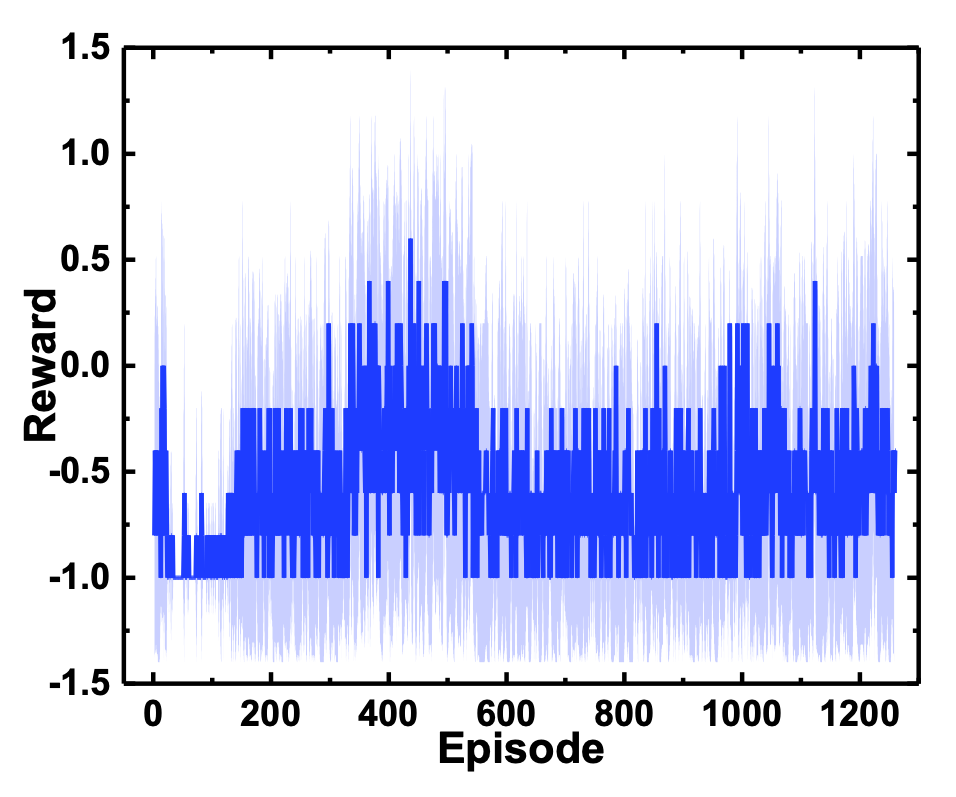
\includegraphics[width=\linewidth]{figure/chapter3/rew=01_obs=面積重心_origin}
        \subcaption{State: area of target, time difference of the area; Reward: success=1, failure=-1, others=0.}
        \label{fig:報酬離散}
    \end{minipage}
    \hspace*{\fill}
    \begin{minipage}[t]{0.45\linewidth}
        \centering
        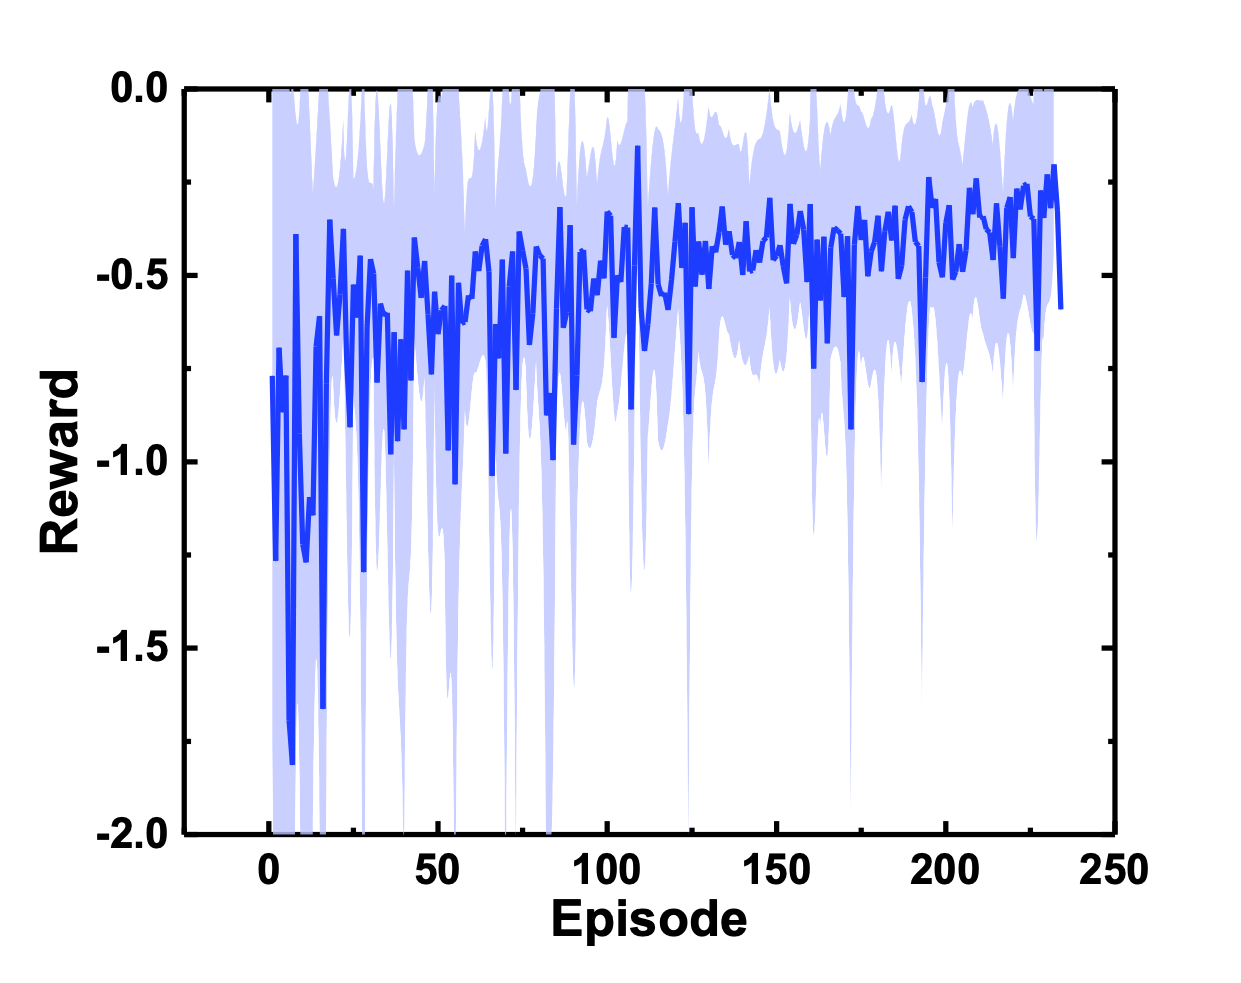
\includegraphics[width=1.1\linewidth]{figure/chapter3/QL_rew=distance_obs=posvec_origin}
        \subcaption{State: relative position; Reward: distance between agent and target.}
        \label{fig:報酬距離}
    \end{minipage}
    \begin{minipage}[t]{0.5\linewidth}
        \centering
        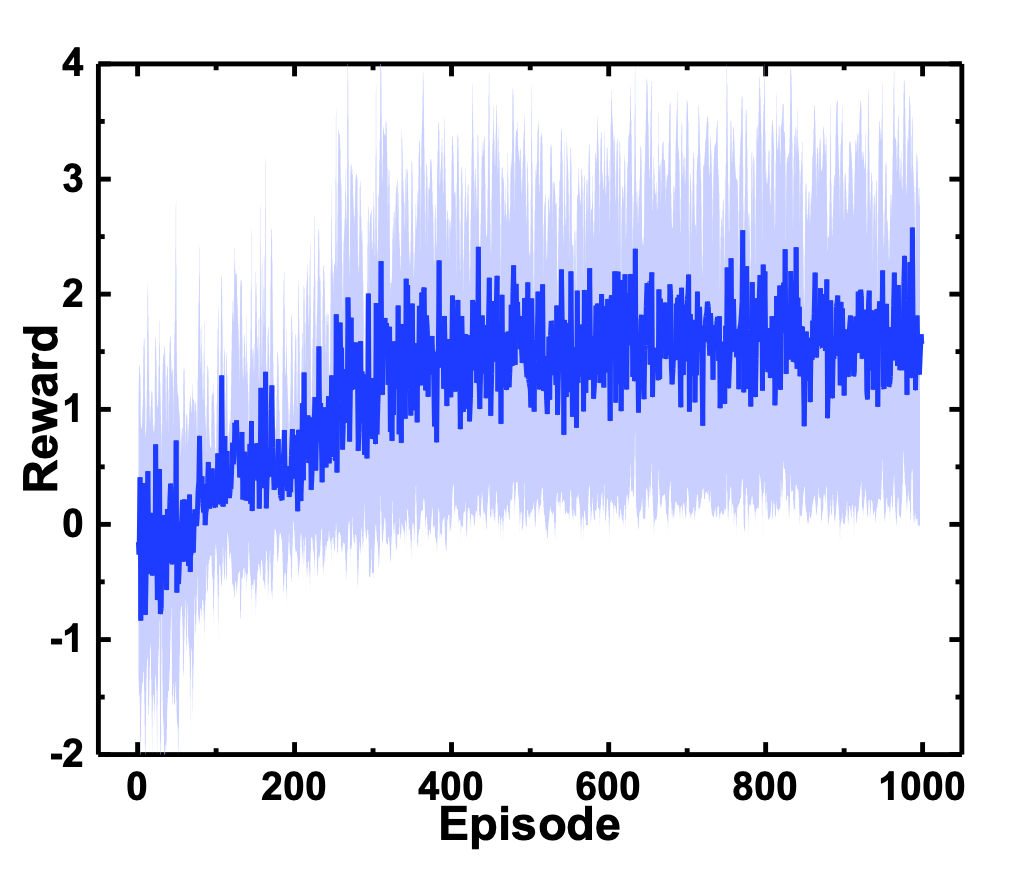
\includegraphics[width=0.95\linewidth]{figure/chapter3/QL_rew=redArea_obs=posvec_origin}
        \subcaption{State: relative position; Reward: area of target.}
        \label{fig:報酬面積}
    \end{minipage}
    \caption{Learning curve of each state and reward at simulation.}
    \label{fig:シミュレーション結果}
\end{figure}


\subsection{考察}
結果を踏まえると,報酬はタスクの成否にあまり関係なく,環境を正しく観測することが重要だということが分かった.\fig{報酬離散}の状態は言い換えると一人称視点であり,\fig{報酬距離},\fig{報酬面積}は環境を俯瞰して見る三人称視点である.三人称視点では自分の周囲の環境全体を観測することができるが,一人称視点では自分が向いている方向しか観測できない.すなわち,探索をしていく中でターゲットを捉えることが必然的に少なくなり,報酬による行動の評価が難しくなる.したがって,一人称視点では中々学習が進まず,三人称視点ではスムーズに報酬が飽和し,学習が完了したと考えられる.


\section{まとめ}
自己完結型の自律駆動ロボットハンドを実現するため,全てのシステムを人間の手のサイズに収容することを目指してスマートフォンのCPU,アクチュエータ制御インターフェースとスマートフォンのカメラ(環境認識)を用いたロボットハンドを作製した.
指定した色(赤色)の物体を認識し,接近し,把持するという一連の動作を行システムを開発し,ターゲットに接近し把持することに成功した.実機での学習とシミュレーション環境での学習を両方行い,外部環境をどう状態に落とし込み状態とするかが学習に大きく関わることを示した.そして,接近タスクにおいてはロボットハンド視点では学習が収束せず,ロボットハンド視点と共にターゲットを俯瞰する視点を併用して観測すると正しく学習できることがわかった.

1号機の課題として以下が挙げられる.
機械的な自由度が少なく,様々な形状の物体を持ち上げて運ぶことが難しい.
様々な種類の物体を識別できない.
AndroidのスマートフォンではPythonから制御すると内蔵カメラの動画が使えず,リアルタイム性に欠ける.
スマートフォンの計算リソースでは重い画像処理が不可能である.

今後は,物体を把持した後に次の行為を実行させるため,より自由度を上げ複雑な動作を可能にするロボットハンドを開発する事の必要性を実感した.ロボットの制御精度と動作速度向上には,環境を認識するセンサとして,環境を俯瞰する位置に定点カメラを設置したり,作動環境内に測距センサを配置する必要がある.加えて,把持対象物が複数ある場合に,使用者が意図する物体を正しく認識し把持できる物体識別性能が重要になってくる.


\section{ヒアリングの実施}
茨城県立大学付属病院リハビリテーション科にて義手使用患者へヒアリングを行い,ロボットハンド1号機の感想をいただいた.
\begin{itemize}
    \item "軽いと感じた"
    \item "家に帰ったらテーブルの上で作業することが多いから,ロボットハンドの有用性はあると思う"
    \item "自分のスマートフォンでできるのが良い"
    \item "クラウドを使わないから停電になったときでも使えて良い"
\end{itemize}
このように義手使用患者からも好評であり,本システムの実用性は高いと考える.
 % 実験手法
\chapter{試作2号機:インスタンス認識ハンド}
\newpage

\section{要求仕様}
1号機の課題の中で特に,把持機構の自由度が小さい事と,物体の正確な識別が不可能である問題は実用化の障害となる.
そこで2号機ではこれら2点の課題を克服したロボットハンドを開発する.

ハードウェアとして,1号機では対象に近づきグリップすることをゴールとしたが,実使用を考えると物を持ち帰って次の動作をすることが要求される.そこで2号機では手首機構を重視して,より多彩な動きを実現するためアクチュエータを増やし,把持機構の自由度を上げる必要がある.グリッパとして,指定した点で掴む,またグリッパの中心軸で左右対称に掴む,という動作を可能にする機構が必要である.また,掴む時の把持点決定及び指定した点を掴めるようアクチュエータで調整できることが要求される.そして掴んだ後の物体の滑り防止機構が必要である.
物体をピックアップするために,環境把握に加えて物体との距離を正確に捉える必要がある.

ソフトウェアとして,1号機に搭載したスマートフォンでは環境認識に1秒を要したため,より高速に演算できる計算リソースが要求される.多自由度化に伴いより多くのアクチュエータを制御するため,スマートフォンではなくGPUを搭載したデバイスで学習・推論を行う必要がある.また,1号機では色のみの認識であったが,把持対象物を"物体"として認識し,複数種類に拡張して識別できることが要求される.


\section{機構設計・機体デザイン}
環境把握と対象物との距離を測るためにRGBカメラとデプスカメラを両方搭載したIntel社のRealSenseを用いた.
対象物を持ち上げるために腕に関節を1つ加え,地面から垂直に対象物を挙上できるようにした.
把持中心点を正確に掴むため,2指対立タイプの一般的な形状のグリッパとした.
把持中心位置の制御では,高精度化のためにラック\&ピニオンを用いてサーボモータの回転を水平運動に変換にし,腕を進行方向と垂直な方向にスライドできるようにした.

以上を考慮して\fig{2号機CAD}に示すようなフレームを3DCAD(123D Design Autodesk社を使用)で設計した.また,ロボットハンドの向きは\fig{2号機向き}に示す,ソフトウェアでの画像(配列)の向きと同様の定義とする.

\begin{figure}
    \centering
    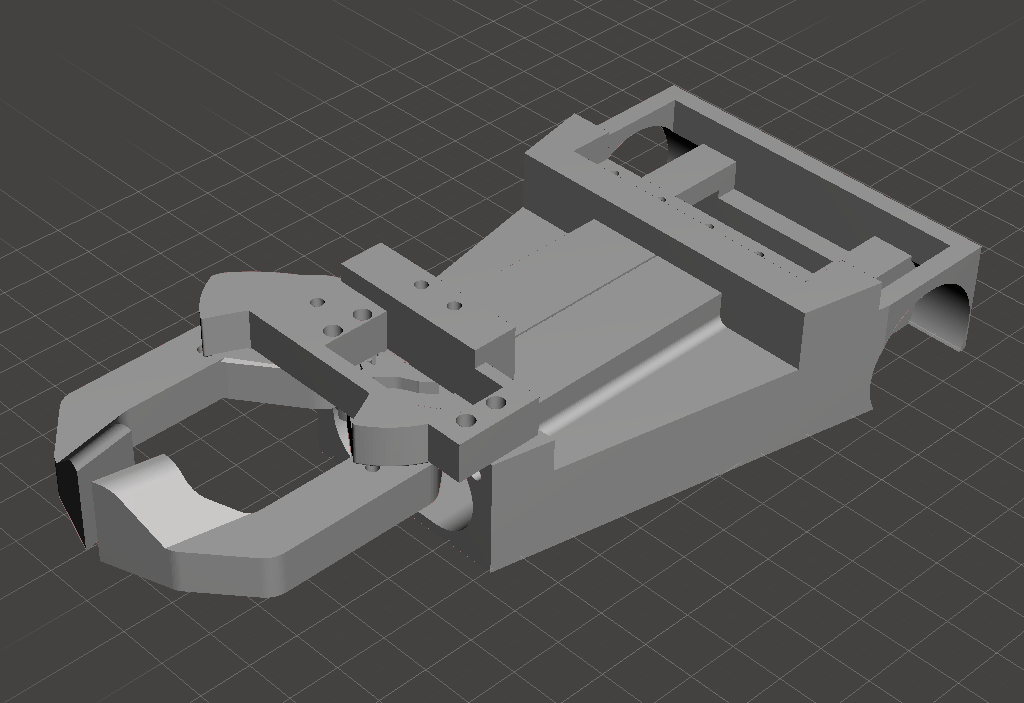
\includegraphics[width=\linewidth]{figure/chapter4/2号機CAD前}
    \caption{3DCAD image of prototype No.2}
    \label{fig:2号機CAD}
\end{figure}

% 向きはここで定義する.CADの写真を使って向きを定義する.

\section{実機作製}

\tab{2号機部品}に2号機作製に当たって使用した部品をまとめた.

\begin{table}[H]
    \centering
    \caption{Components of prototype No.2}
    \begin{tabular}{cc}\toprule
        本体フレーム & PLA(赤) \\
        デプスカメラ & RealSense D435i \\ 
        マイコン & Arduino Nano \\ 
        DCモータ & \href{http://akizukidenshi.com/catalog/g/gM-12379/}{STLギヤモータ 栄42D長軸型} \\ 
        サーボモータ & \href{https://hitecrcd.co.jp/products/servo32225/}{HS-225MG} x1,\href{https://hitecrcd.com/products/servos/discontinued-servos-servo-accessories/hsr-5990tg-hmi-ultra-premium-robot-servo/product}{HSR-5990TG} x1,\href{https://hitecrcd.co.jp/products/servo31422s/}{HS-422} x1 \\ 
        バッテリー & モバイルバッテリー \\ 
        タイヤ & \href{https://tamiya.com/japan/products/70194/index.html}{TAMIYA製スパイクタイヤ} \\
        リニアガイド &  \\
        ラック\&ピニオン &  \\ \bottomrule
    \end{tabular} 
    \label{tab:2号機部品}
\end{table}

1号機と同様にロボットハンドのフレームは簡便さと軽さを考慮して3Dプリンタ(Adventure3)で造形した.
\fig{2号機外観}に作製したロボットハンドの外観を示す.

2号機の総重量は572.27gであった.

\begin{figure}
    \centering
    \begin{minipage}{\linewidth}
        \centering
        \includegraphics[width=\linewidth]{figure/chapter4/2号機外観}
        \caption{Appearance of Prototype No.2. Weight is 572.27 g.}
        \label{fig:2号機外観}
    \end{minipage}
    \begin{minipage}{\linewidth}
        \centering
        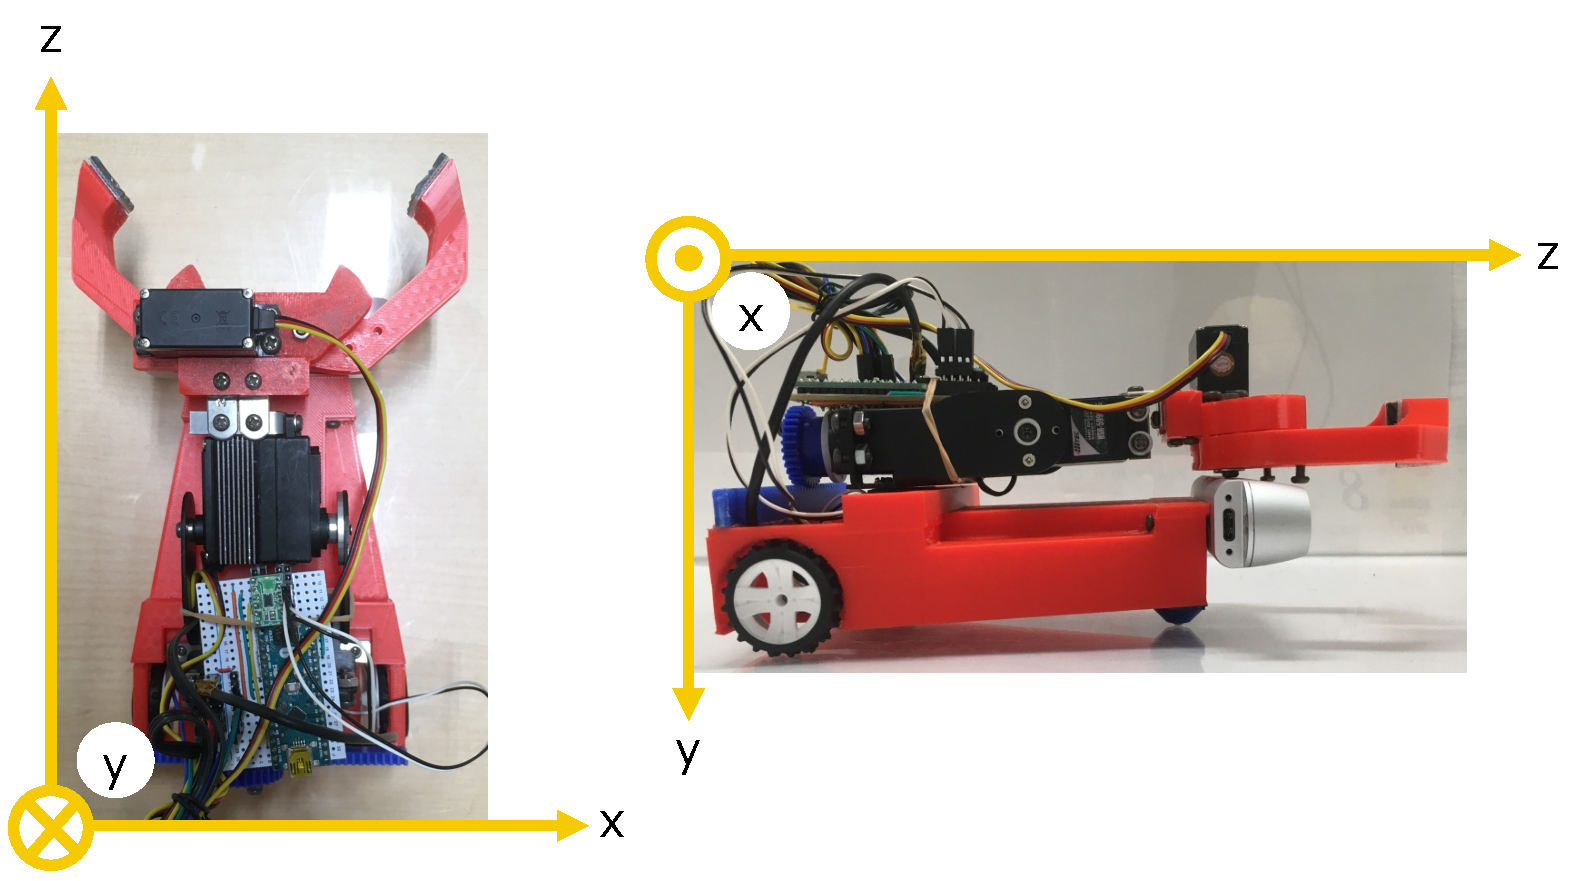
\includegraphics[width=0.9\linewidth]{figure/chapter4/2号機向き}
        \caption{Definition of orientation at prototype No.2}
        \label{fig:2号機向き}
    \end{minipage}
\end{figure}


\section{制御アルゴリズム}
2号機では強化学習ではなく比例制御の考え方を利用した手法及びルールベースによって対象物のピックアップを行う.

接近動作では2段階に分けて行う.まず対象物までのラフな接近について述べる.
対象物のマスクを取得し重心を計算する.その重心がロボットハンドの中心軸に来るように左右輪のスピードをそれぞれ独立に以下の更新式によって制御しながら接近する.

\begin{lstlisting}[caption=接近アルゴリズム, label=code:motor]
    r_motor = (1 - error_distance) / 2 * MAX_SPEED
    l_motor = (1 + error_distance) / 2 * MAX_SPEED
\end{lstlisting}

ここで\texttt{MAX\_SPEED}はモーターの最大スピードで今回は100とした.\texttt{error\_distance}はロボットハンドと対象物との画像内におけるx軸方向のズレを画像の横の長さで規格した値であり,-1から1の値をとる.そして対象物から20cmまで近づいたら停止させる.

次に,対象物の重心にハンドの把持中心が来るように横方向にラックピニオンで修正を加える.この時,画像におけるピクセル間距離を実距離に変換し重心とハンド中心の変位をなるべく小さくするようにサーボを動かす.そしてデプスカメラが対象物に覆われて見えなくなるまで直進する.
そこからさらに4cm直進しグリッパーを閉じる.その後腕を上げ物体を持ち上げ,この際のデプス画像を保持しておく.そこから1秒ごとにデプス画像の現フレームとのピクセル数比を取り,50\%以下であったら失敗とし,5秒落とさず維持したら把持成功とした.

把持が成功したらホームポジションまでコード\ref{code:motor}と同様の制御で戻る.ホームポジションの認識にはARマーカーを使用した.

なお,Arduinoとのシリアル通信では1回に2byteまでしか送信できず,String型でモーター5つの情報を送信すると遅延や読み飛ばしが発生した.そこで2号機ではモーターの取る値をデジタル化し情報を圧縮してByte型で送信するようにした.実際に取る値と送信bit信号の対応表を\tab{2号機信号表}に示す.

\begin{table}
    \centering
    \caption{}
    \begin{tabular}{cccc}\toprule
        Actuator & Bit serial & Value @ Arduino & Value @ Python \\ \midrule
        Forward right DC motor & 000 & 0--100(step 5) & 0--20  \\ 
        Forward left DC motor & 001 & 0--100(step 5) & 0--20 \\ 
        Grip servo & 010 & 0 / 100 & 0 / 1\\ 
        Vertical swing servo & 011 & 0 / 100 & 0 / 1 & 011 \\ 
        Horizontal slide servo & 100 & 0--180 (step 10) & 0--18 \\ 
        Terminate & 101 & 0 / 1 & 0/1 \\ 
        Backward right DC motor & 110 & 0--100(step 5) & 0--20 \\ 
        Backward left DC motor & 111 & 0--100(step 5) & 0--20 \\ \bottomrule
    \end{tabular} 
    \label{tab:2号機信号表}
\end{table}

Bit serialが駆動させるアクチュエータを2進数で示しており,動かす値をValue @ Pythonに示す10進数を5桁の2進数に変換してそれぞれをドッキングして8桁の2進数としてシリアル送信する.


デプスカメラおよびArduinoの制御はG-DEP社のDeepLearning BoxII(Ubuntu16.04)を使用し,計算リソースはNVIDIA社のGPU(TITAN RTX)を使用した.
プログラムは以下のURLの筆者のGitHubで公開している.
\url{https://github.com/yumion/onodera-lab/tree/master/robotHandV2}


\subsection{デプスカメラを使用したカメラ画像内における実距離推定}
把持位置を制御する際,画像内の実際の長さ知る必要がある.そこで,ピクセル間距離から実距離を回帰処理によって求めた.また,カメラから測る対象物までの距離にも依存するため,デプスカメラを用いて距離依存性についても回帰処理を行い,2段階で求めた.

壁に30cm定規を置き,カメラは壁と平行になるよう設置した.壁からカメラの距離$z$(cm)を変えながら定規の目盛りのピクセル座標を取得し,横軸にピクセル差分$\Delta \rm{pixel}$,縦軸にそのピクセルに対応する定規の目盛り幅$\Delta x$(cm)をプロットした(\fig{pix2dist}).また,各$z$で線形回帰を行ったあと横軸に壁からカメラの距離$z$,縦軸に傾き$a$をプロットし線形回帰を行い,全ての距離$z$におけるピクセル間距離を求めた(\fig{depth2grad}).


\begin{figure}[H]
    \centering
    \begin{minipage}{0.45\columnwidth}
        \centering
        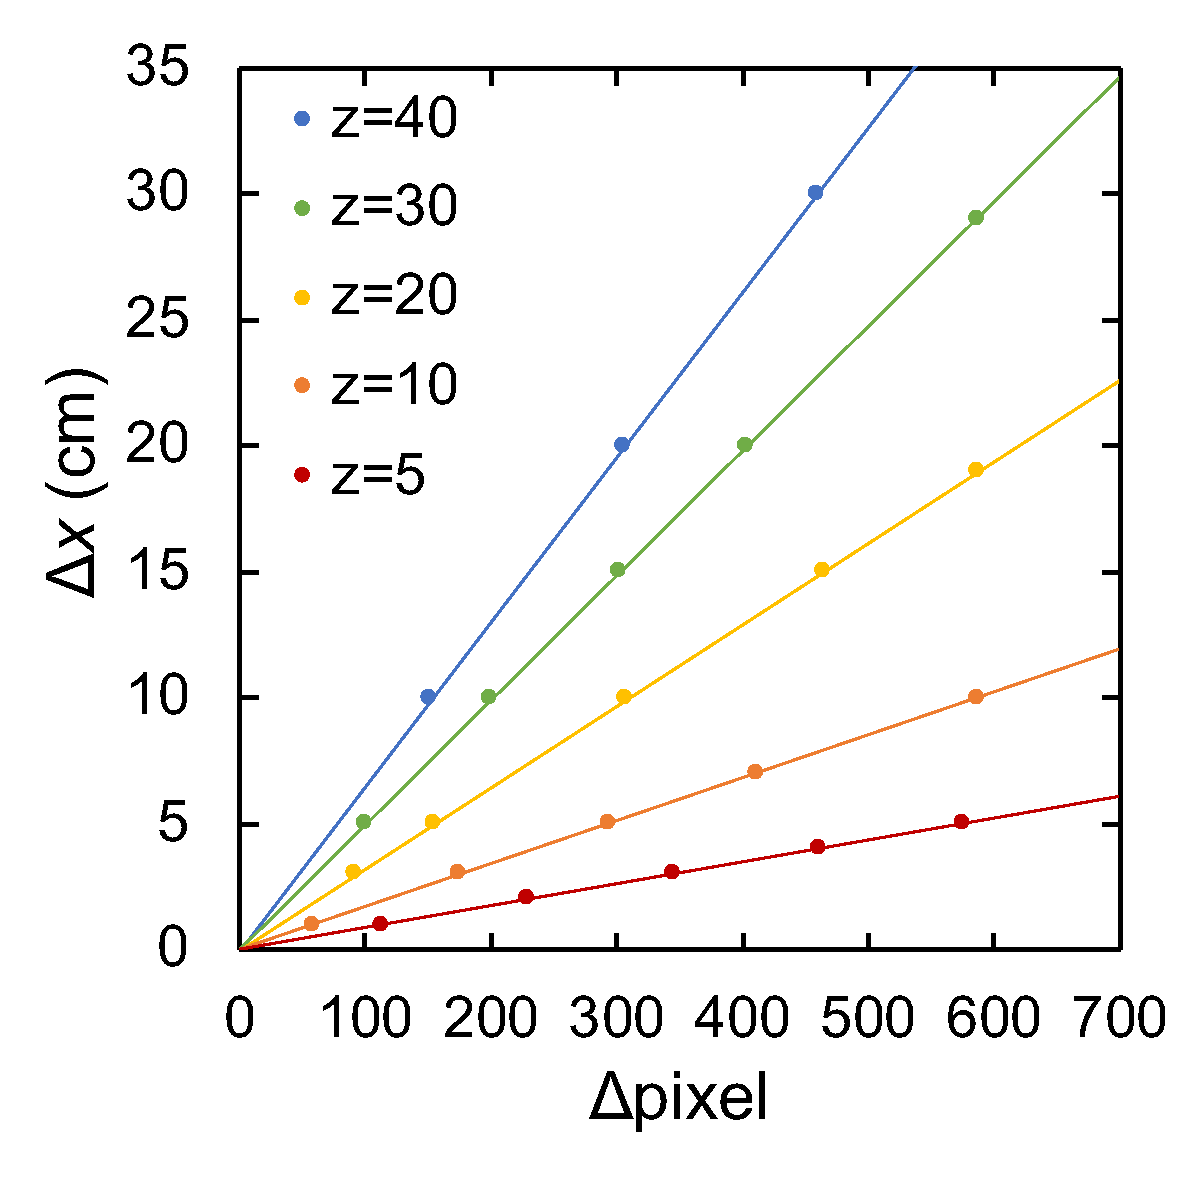
\includegraphics[width=\linewidth]{figure/chapter4/pixel2distance}
        \subcaption{Pixel to Distance}
        \label{fig:pix2dist}
    \end{minipage}
    \begin{minipage}{0.45\columnwidth}
        \centering
        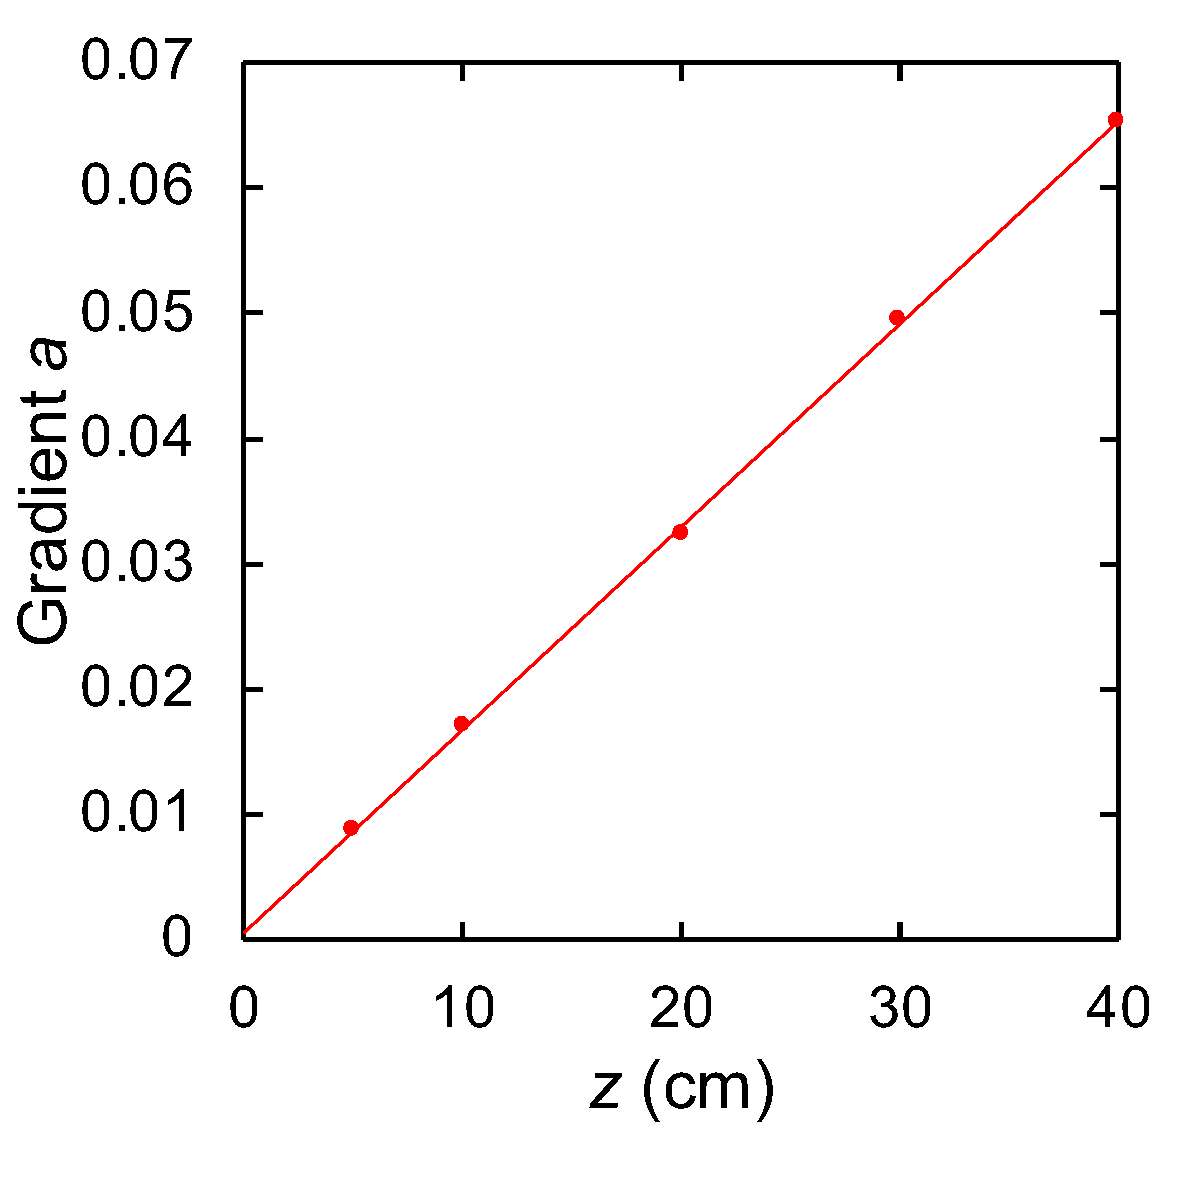
\includegraphics[width=\linewidth]{figure/chapter4/depth2gradient}
        \subcaption{Dependency of depth}
        \label{fig:depth2grad}
    \end{minipage}
    \caption{Convert pixel-wise to distance in real.}
    \label{fig:pix2distance}
\end{figure}


\begin{figure}[H]
    \centering
    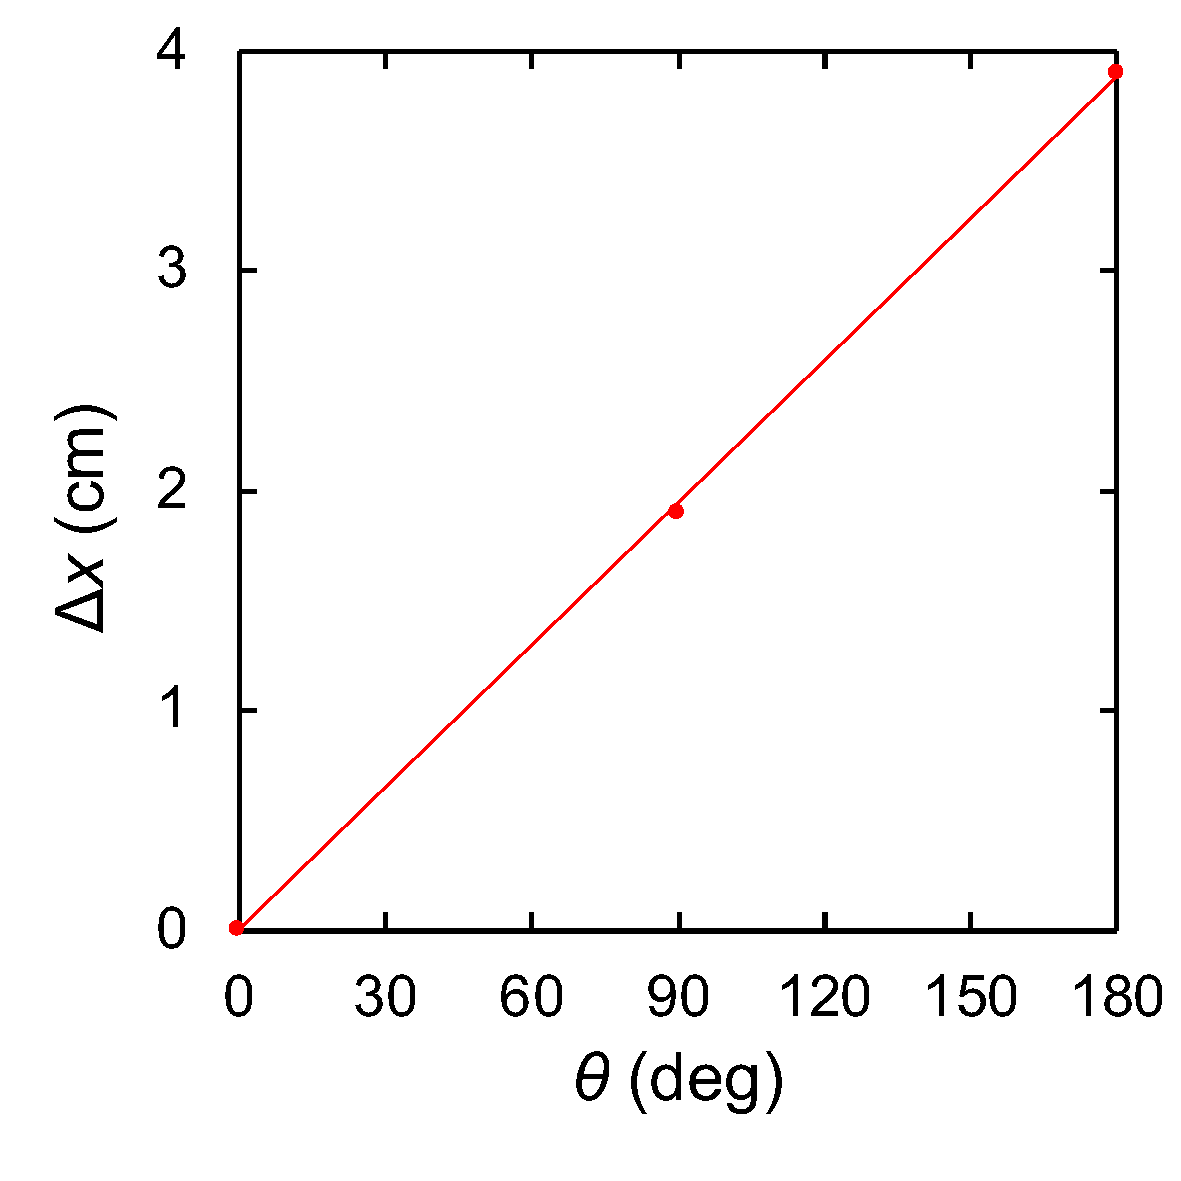
\includegraphics[width=0.5\linewidth]{figure/chapter4/servo2distance}
    \caption{Convert servo input to distance.}
    \label{fig:servo2dist}
\end{figure}

以上から,実距離$\Delta x$はピクセル間距離$\Delta \rm{pixel}$とカメラと対象物の距離$z$を用いて
\begin{align}\label{eq:ピクセル間距離}
    \Delta x \simeq (0.0016z + 0.0006) \cdot \Delta \rm{pixel}
\end{align}
と推定できる.

また,ラック\&ピニオンの回転から水平移動に変換するためには,サーボが0\deg -- 180\deg まで可動するため,その移動最大距離を測定しておき(4cm),各角度における0\deg からの移動量をプロットし線形回帰する(\fig{servo2dist})ことで以下のように求められる.

\begin{align}\label{eq:スライド角度}
    \Delta x \simeq 0.0216 \theta
\end{align}
ここで,$\Delta x$は水平移動距離(cm),$\theta$はサーボの回転角度(deg)である.
\eq{ピクセル間距離}と\eq{スライド角度}から
\begin{align}
    \theta & \simeq \dfrac{\Delta x}{0.0216} \\
           & = \dfrac{0.0016z + 0.0006}{0.0216} \Delta \rm{pixel} \\
\end{align}
として画像からサーボを何度動かせば良いかが分かる.なお,実装上はサーボの可動範囲が0\deg -- 180\deg を考慮して
\begin{lstlisting}[label=code:servo]
    vertical_deg =\
        (max(min(vertical_pos // 0.0216, 90), -90) + 90) // 10
\end{lstlisting}
とすることで入力の最小0,最大を180とし,サーボへの入力が0の時に真ん中である90\deg とし,それを1/10にデジタル化して送信する.\texttt{vertical\_pos}は$\Delta x$(cm),\texttt{vertical\_deg}は$\theta$(deg)である.


\subsection{Mask R-CNNを用いた物体のセグメンテーションと測距}
Instance Segmentationの手法の1つであるMask R-CNNを用いた.MSCOCO2014および2017のデータセットで学習した.
学習した結果を\tab{MSCOCO評価}に示す.

\begin{table}[H]
    \centering
    \caption{Results of Mask R-CNN validated by COCO.}
    \begin{tabular}{ccccc}\toprule
        & \multicolumn{2}{c}{Object Detection} & \multicolumn{2}{c}{Segmentation} \\ 
         & 2014 & 2017 & 2014 & 2017 \\ \midrule
        $\rm{AP}^{\rm{IoU}=0.50:0.95} \u{maxDets=100} @Area=all$ & 0.352 & 0.227 & 0.334 & 0.243 \\ 
        $\rm{AR}^{\rm{IoU}=0.50:0.95} \u{maxDets=100} @Area=all$ & 0.438 & 0.299 & 0.405 & 0.301 \\ 
        FPS & 4.078 & 3.880 & 4.013 & 4.002 \\ \bottomrule
    \end{tabular} 
    \label{tab:MSCOCO評価}
\end{table}

また,デプスカメラを用いて検出した物体の距離も同時に測定した.Mask R-CNNの出力であるマスクの重心を求め,その座標までの距離をデプスカメラで測定した.\fig{maskrcnn例}に学習済みモデルを使用した物体検出およびその物体までの測距の例を示す.

\begin{figure}[H]
    \centering
    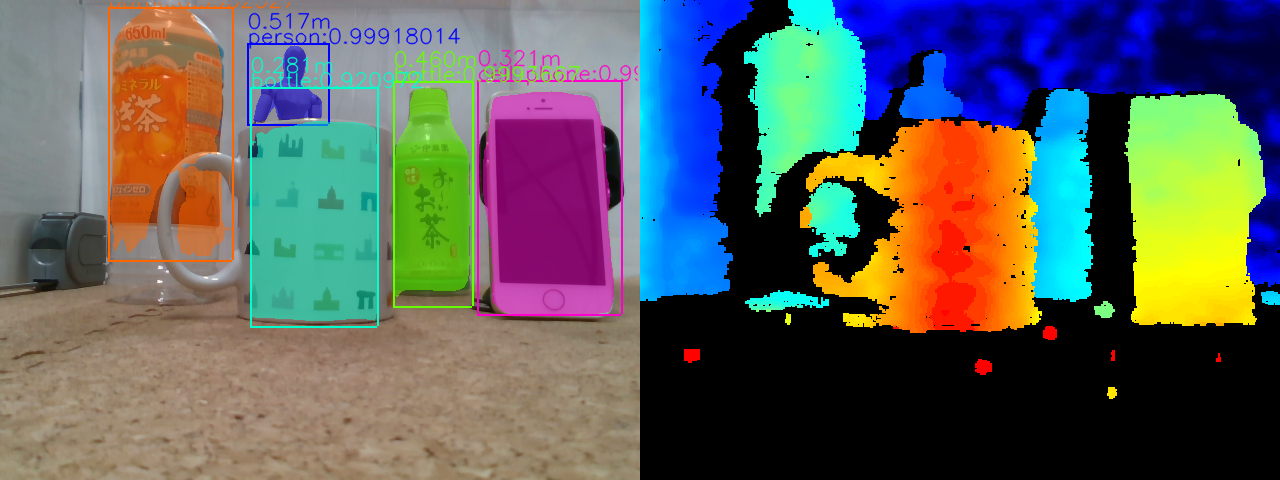
\includegraphics[width=0.7\linewidth]{figure/chapter4/MaskR-CNN_screenshot}
    \caption{Examples of Mask R-CNN inference.}
    \label{fig:maskrcnn例}
\end{figure}


このように,マスクが完璧出なくとも対象物の重心はおおよそ把握できるため,IoUよりもPrecisionを重視し物体検出におけるFPSが高い2014年学習モデルを使う.


\section{評価方法}
今回2号機でアップデートしたのは,対象物の識別と把持動作であったため,この2点に関して評価を行う.

MSCOCOデータセットの中で,机の上にあるものを識別・把持できるかを検証した.
今回,対象とした物体は\fig{対象物}に示す5つの物体(4種類)である.また,\tab{対象物}に各対象物の詳細を示す.
\begin{figure}[H]
    \centering
    
    \begin{minipage}{0.19\columnwidth}
        \centering
        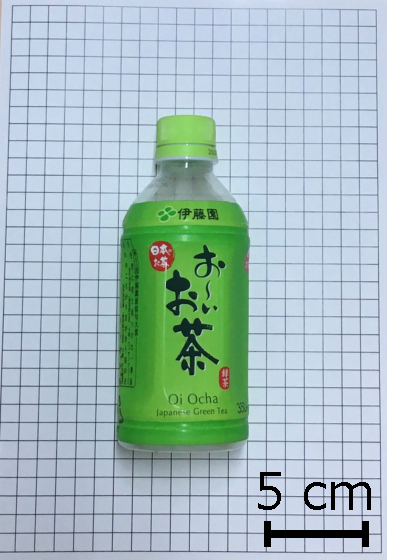
\includegraphics[clip, width=\linewidth]{figure/chapter4/bottle_350ml}
        \subcaption{bottle(350ml)}
    \end{minipage}
    \begin{minipage}{0.19\columnwidth}
        \centering
        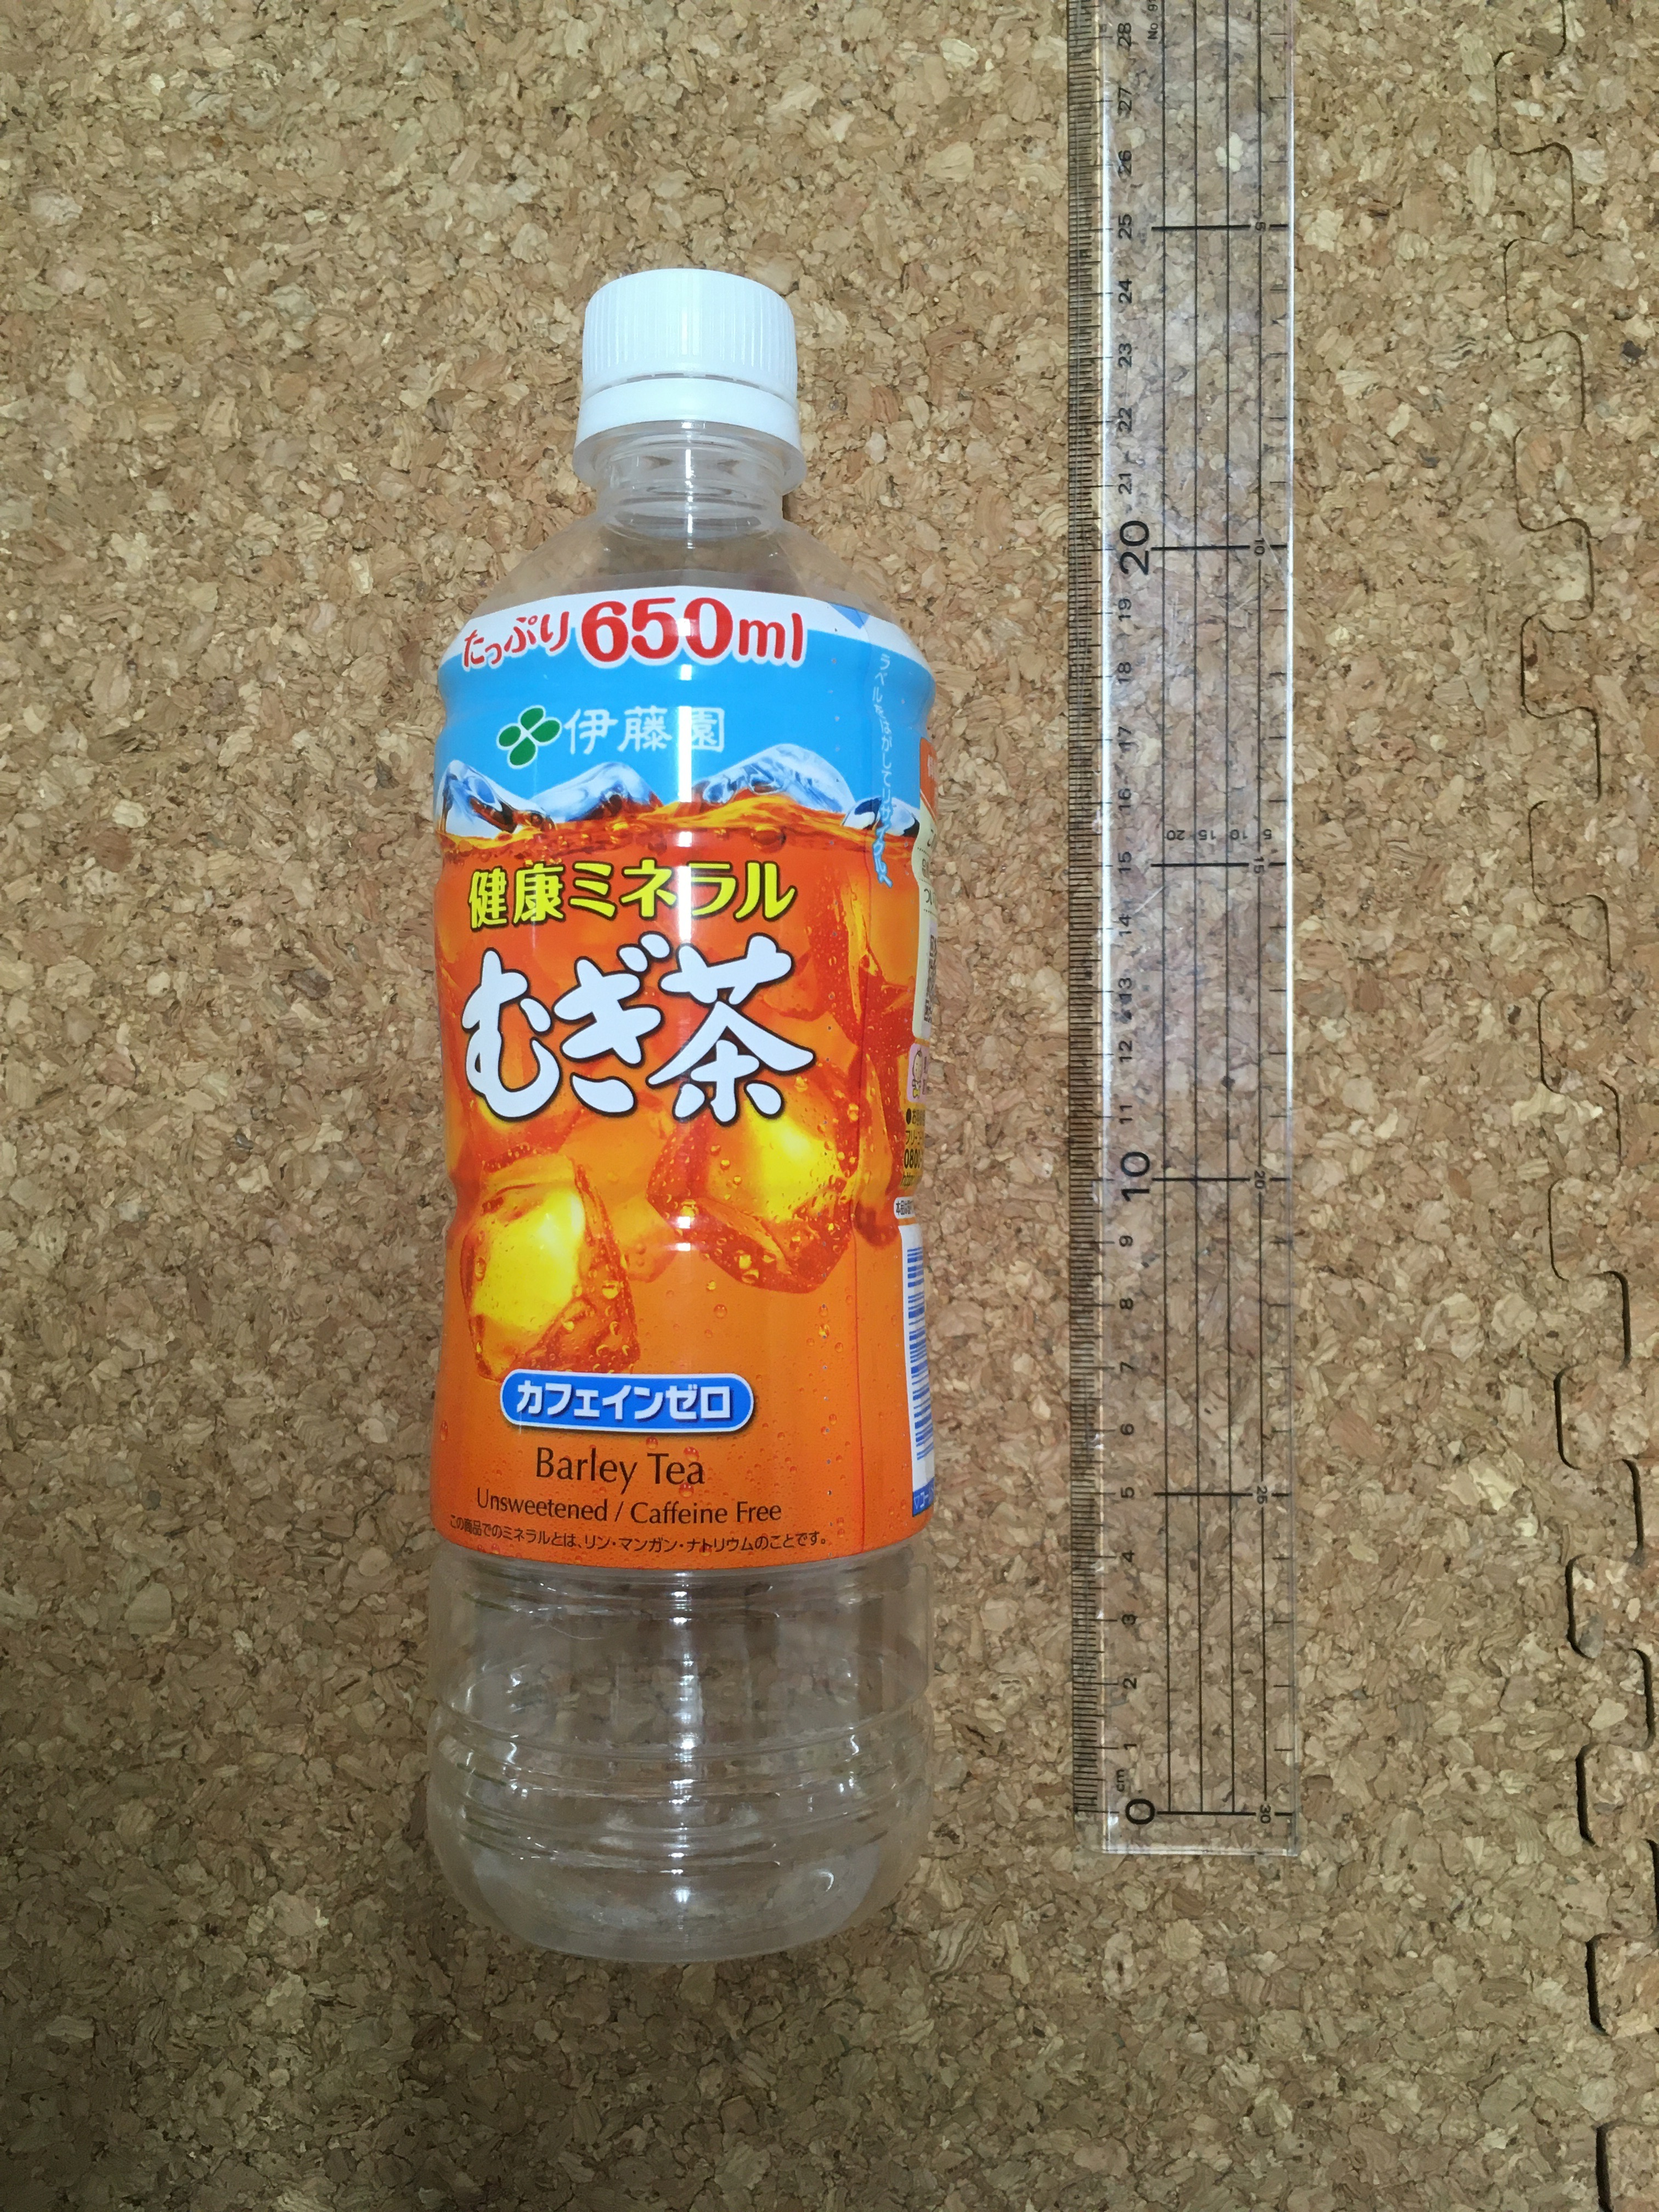
\includegraphics[clip, width=\linewidth]{figure/chapter4/bottle_650ml}
        \subcaption{bottle(350ml)}
    \end{minipage}
    \begin{minipage}{0.19\columnwidth}
        \centering
        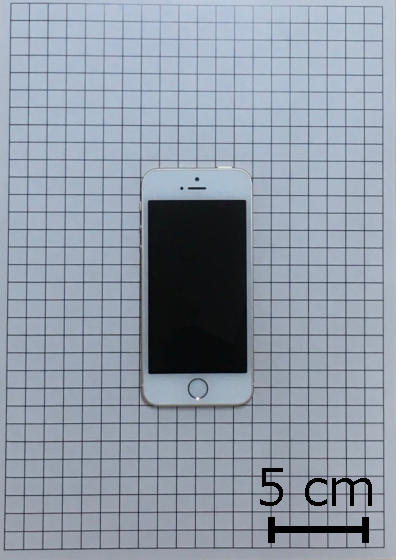
\includegraphics[clip, width=\linewidth]{figure/chapter4/cellphone}
        \subcaption{cell phone}
    \end{minipage}
    \begin{minipage}{0.19\columnwidth}
        \centering
        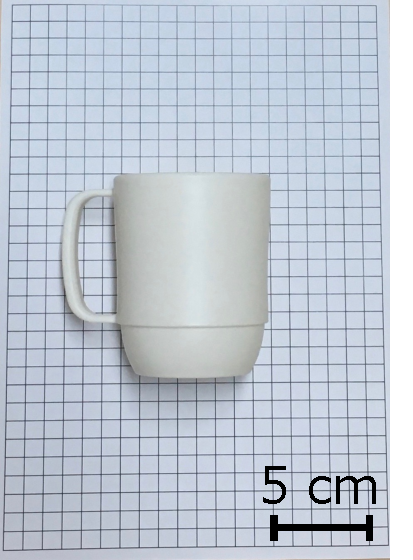
\includegraphics[clip, width=\linewidth]{figure/chapter4/cup2}
        \subcaption{cup}
    \end{minipage}
    \begin{minipage}{0.19\columnwidth}
        \centering
        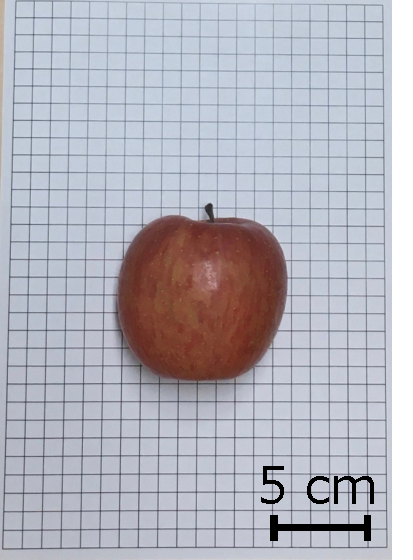
\includegraphics[clip, width=\linewidth]{figure/chapter4/apple}
        \subcaption{apple}
    \end{minipage}

    \caption{Objects.}
    \label{fig:対象物}
    
\end{figure}

\begin{table}[H]
    \centering
    \caption{Details of objects.}
    \begin{tabular}{ccccc}\toprule
        & Size & Weight & \# of Training data & Notes \\ \midrule
        bottle(350 ml) & 16.5 $\times$ $\phi$ 5.9 cm & 26.28 g & \multirow{2}{*}{8880} & Empty \\ 
        bottle(650 ml) & 22.0 $\times$ $\phi$ 6.9 cm & 29.94 g &  & Empty \\ 
        cell phone & 0.78 $\times$ 5.9 $\times$ 12.0 cm & 127.51 g & 5017 & iPhone SE \\ 
        cup & 9.8 $\times$ $\phi$ 7.9 cm & 82.50 g & 9579 & Empty \\ 
        apple & $\phi$ 8 cm & 263.32 g & 1662 & Raw \\ \bottomrule
    \end{tabular}
    \label{tab:対象物}
\end{table}

まず,学習済みモデルを使用してMask R-CNNの識別精度を検証した.また各対象物において,ロボットハンドとの距離すなわち画角によってMask R-CNNの検出精度およびそのクラス分類の精度が異なるかを検証した.

次に,各物体に対して接近成功率および把持成功率を検証した.接近成功率とは,対象物の17cm以内に近づきかつ対象物を正面に捉えて静止したら成功,対象物の正面で止まれなかったら失敗とし,10回試行したときの成功率とする.把持成功率とは5秒間持ち上げ続けたら成功,そうでなければ失敗とし,10回試行したときの成功率とする.
接近および把持のタスクは以下のように定めた.タスク1が接近タスクでタスク2が把持タスク,タスク1+タスク2が接近・把持の一貫タスクである.
\begin{itemize}
    \item タスク1\\
    離れたところに対象物を置き,17cm以内まで接近する.
    \item タスク2\\
    対象物の向かい17cmの場所から把持を行う.
    \item タスク1+タスク2\\
    離れたところに対象物を置き,17cm以内まで接近し,そこから把持を行う.
\end{itemize}


\section{結果}
\subsection{識別性能評価}
"bottle"はどの向きにおいても検出できた."cell phone"はエッジ部分だけでは検出できず,画面側か背面のみ検出できた."cup"は取っ手が写っている角度では検出できたが,取っ手が写らない向きになると"bottle"と誤認識することがあった."apple"はどの向きにおいて認識できなかった.

各対象物において,識別精度の対象物依存性を\fig{mrcnn距離}に示す.なお,"apple"は全ての場所・向きにおいて認識できなかったため載せていない.
\begin{figure}[H]
    \centering
    \begin{minipage}{0.45\columnwidth}
        \centering
        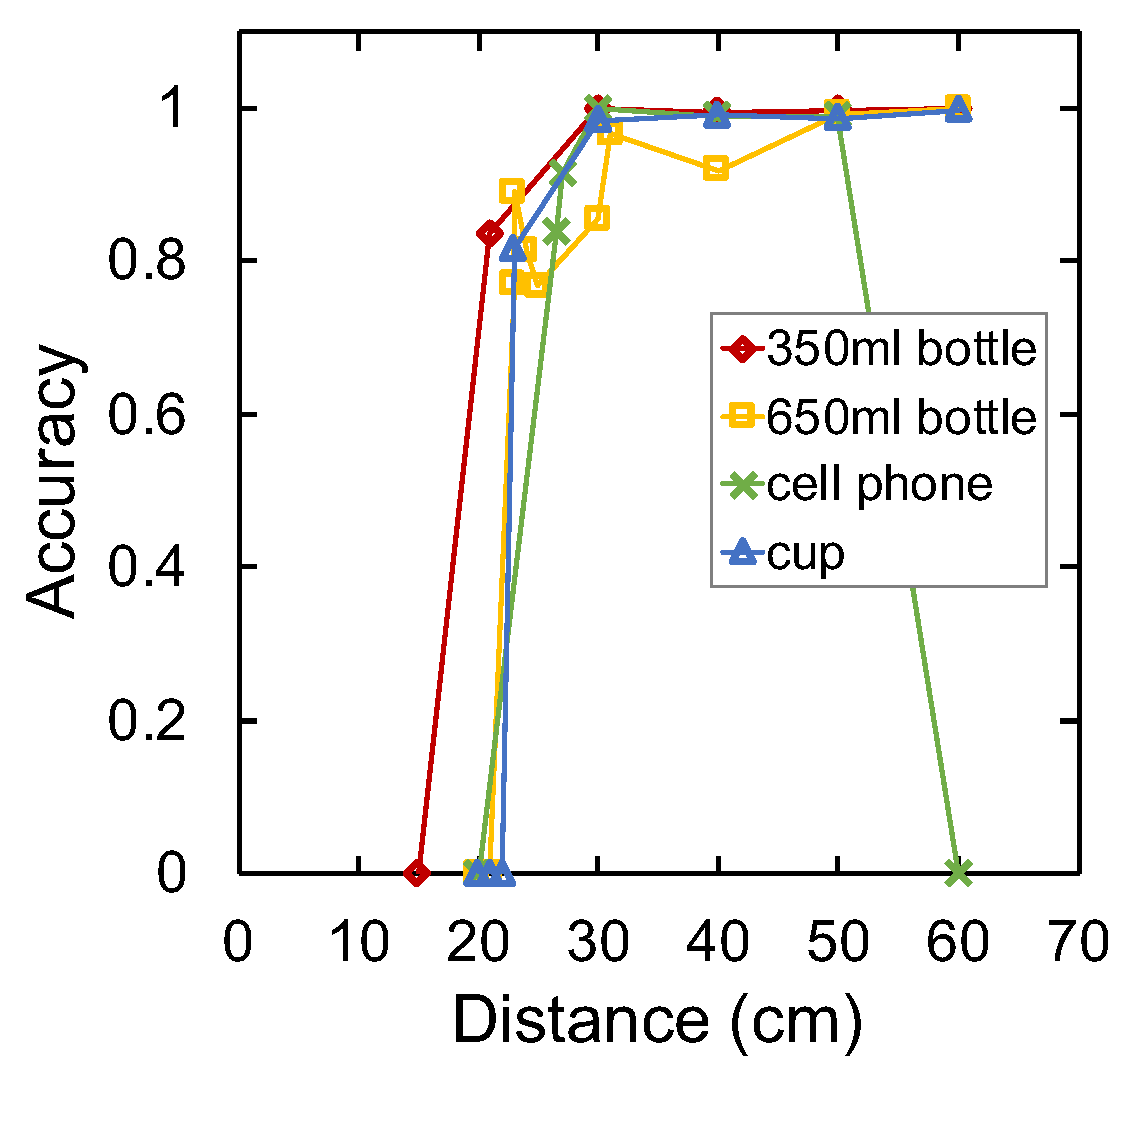
\includegraphics[width=0.95\linewidth]{figure/chapter4/mrcnn_depth}
        \subcaption{Input raw image.}
        \label{fig:mrcnn距離そのまま}
    \end{minipage}
    \begin{minipage}{0.45\columnwidth}
        \centering
        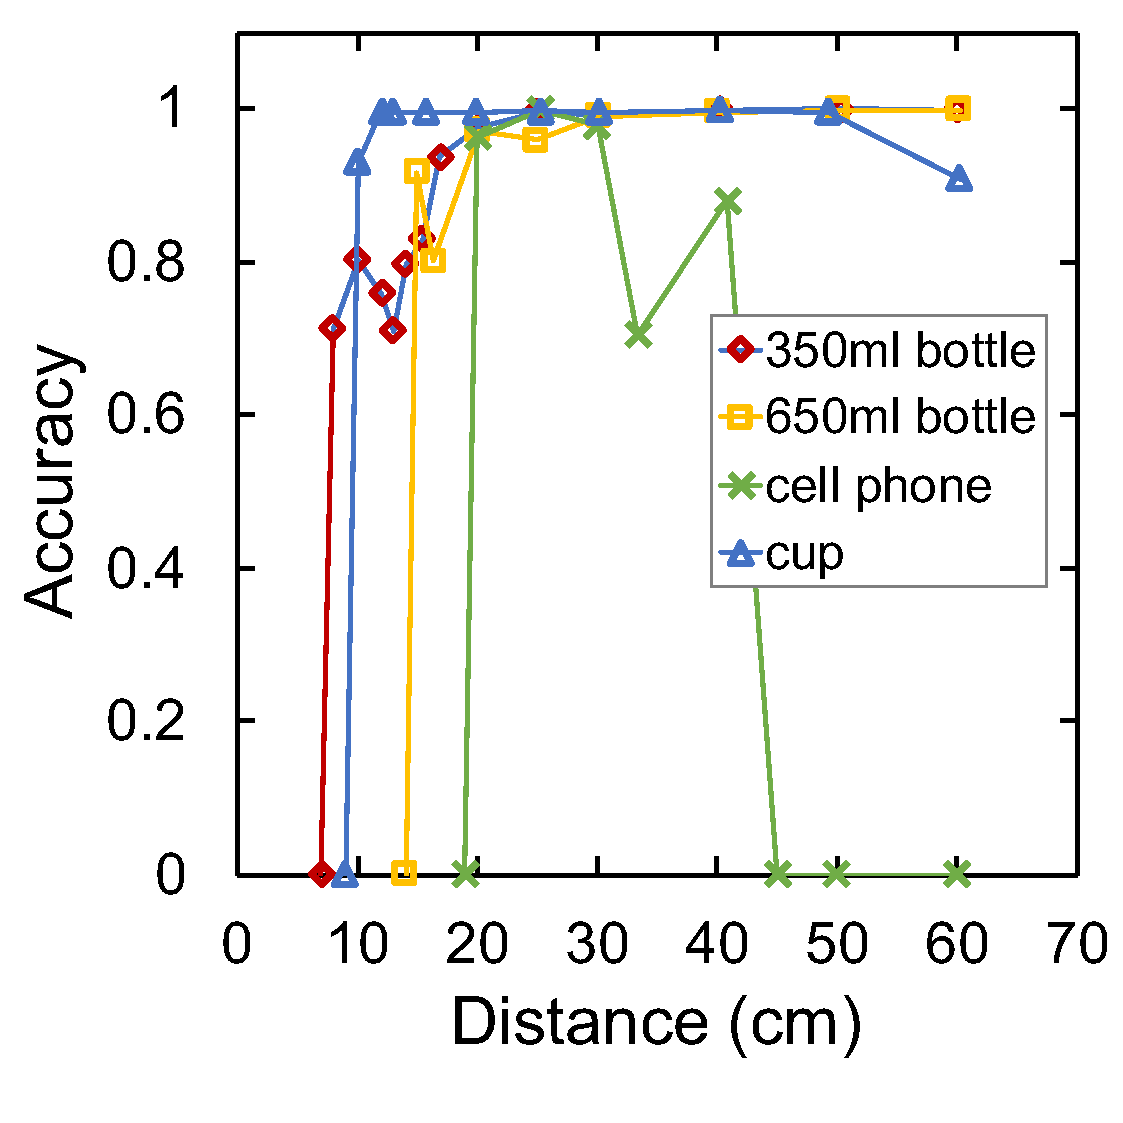
\includegraphics[width=0.95\linewidth]{figure/chapter4/mrcnn_depth_padding}
        \subcaption{Input zero padding image.}
        \label{fig:mrcnn距離パディング}
    \end{minipage}
    \caption{Dependency of distance between camera and object.}
    \label{fig:mrcnn距離}
\end{figure}
入力にカメラ画像をそのまま入れた結果が\fig{mrcnn距離そのまま}であった.30cmを境に識別精度が落ちていることが分かる.

\subsection{把持タスク評価}


\begin{table}[H]
    \centering
    \caption{Success rate on grasping objects tasks.}
    \begin{tabular}{cccc}\toprule
        Objects & Task1 & Task2 & Task1 + Task2 \\ \midrule
        bottle (350 ml) & 60\% & 90\% & 50\% \\
        bottle (650 ml) & 60\% & 80\% & 50\% \\
        cell phone & 60\% & 50\% & 40\% \\ 
        cup & 70\% & 50\% & 30\% \\ \bottomrule
    \end{tabular} 
    \label{tab:把持成功率}
\end{table}

失敗例は,掴み方が悪く掴んでも落とした,掴んで持ち上げたがロボットハンド自体が横転した,持ち上げたがズレ落ちた,などがあった.

また,ホームポジションに戻る動作も実装した.


\section{考察}
appleが認識できなかった原因は,学習データ数の偏りにあると考えられる.\tab{対象物}に示したように,appleだけ他の対象物よりも訓練データが3分の1以下と少ない.したがって今回使用したモデルはappleの認識が弱いモデルだったと考えられる.

Mask R-CNNの検出精度における対象物との距離依存性では,対象物の高さに関係なく30cmから精度が落ち始め,20cmでは全ての物体で検出できなくなった(\fig{mrcnn距離そのまま}).背の高いbottle(650ml)は,距離が近いと画像内に物体全体が収まらず検出精度が下がると予想できるが,背の低いcupも同じように精度が下がった.これは学習データに大きく写っている画像が無いことが原因と考えられる.
そこで,入力画像をzero paddingして対象物を小さく写るようにして入力した結果が\fig{mrcnn距離パディング}である.paddingをすることで大幅に距離依存性が改善され,17cmまで近づいても検出されるようになった.したがって,接近タスクでは17cmを閾値としてそこまで近くタスクとした.

把持成功率より接近成功率が低い原因は,2号機のRGBカメラの位置だと考えられる.2号機に搭載したカメラRealSenseは左端にRGBカメラ,真ん中右寄りにDepthカメラが付いているため,RGB画像は右側を見ることが難しい.そのため,ロボットハンドから距離が離れていれば問題ないが,物体がロボットハンドに近い位置で右側にいると死角となり,認識できないため接近できないという事になる.また,cell phoneとcupは把持成功率が低く,bottleの把持成功率が高い理由としては,把持対象物の対称性だと考えられる.bottleは円筒対称であるため,どの角度からアプローチしても同様の持ち方で把持が可能だが,cell phoneやcupはbottleより対称性が悪いため,ルールベースでは正しい位置で把持できない.これは各物体に対して把持位置を学習するなど,高度なアルゴリズムが必要となる.

\section{まとめ}
物体の種類を識別し,把持し,元いた位置に運搬することができた.



 % 結果と考察
\chapter{結論}
\newpage

\section{総括}

本論文では,実用的な電動義手の開発を目的として,3D プリントと jamming 転移現象を 活用した義手試作を行った.jamming グリッパのモデル化と,Bio-mimic 吸盤の開発に取り 組み,実際に吸盤構造体を搭載することで,従来の jamming グリッパでは困難とされてい る扁形物体の把持が可能になった.これにより jamming グリッパの能力を向上・拡張する ことに成功した.
義手の試作にあたっては,実際に東京大学医学部付属病院にて実際の義手利用者からヒ アリングを行い,義手の外観が利用者の心理的ならびに QOL の観点から非常に大きなウェ イトを占めているとの知見を得た.そこで,著者自身のリアルな手をモデルにするととも に,人間の手が行う把持機能に注目してプロトタイプを作製した.作製した電動義手は, ローコスト,軽量,耐水性といった特徴を持つとともに,握力把持,精密把持の 2 種類の 方式での把持能力を持っていることを確認した.

本研究ではパーソナルロボットを小型化し,義手使用患者や片麻痺患者など上肢機能障害患者を対象としたパーソナルロボットを開発する.義手は常に身につけているように,パーソナルロボットも携帯できるよう小型化し腕の形をしたロボットハンドとする.上肢機能障害者にとってはパーソナルロボットはどんな事態でも動作する必要があるため,今回はCloudは使用せずEdgeで処理を行うこととする.また座って机で作業することが多いため使用場所を机の上に限定し,指定した物をピックアップするタスクを実行できるパーソナルロボットハンドを作製することを目的とする.





本研究では,上肢機能障害者支援を目指し,強化学習・深層学習をロボット制御に適用した携帯可能な自律型ロボットハンドの試作を行った.

\subsection*{試作1号機}



\subsection*{試作2号機}



\section{今後の展望}
\subsection*{デザインの改善}
地面から直立している物体のみで,平たい物体や細長く自立しない物体などは把持不可能であった.そのため,腕の関節と手首の関節を増やすことで,地面に対して垂直にアプローチできるように改善すると把持できる物体の幅が広がる.また,今回グリッパは大した考慮をしていなかったため,様々な物体を把持可能であるJammingグリッパ\cite{jamminggripper}など,グリッパ形状を検討する必要がある.

\subsection*{ハードウェア(計算リソース)の改善}
2号機では識別能力を向上させるために,外部の計算リソースを使用していたためGPU搭載PCと有線で接続されていたことが大きな課題であった.そこで次世代機ではEdgeデバイスであるJetsonNanoを使用することで,localでもGPUを使用した推論が可能となる.さらにJetsonNanoはanalogWriteができるため,Arduinoを必要とせずアクチュエータの制御が可能となり,よりシンプルな設計にできると考えられる.

\subsection*{ソフトウェアの改善}
接近タスクは比例制御で十分有効であることがわかったが,把持タスクはルールベースでは物体の形状に対称性が無いものは把持成功率が低かった.把持タスクにはVisionベースの教師あり学習を行い最適な把持点を掴むことで改善できる.さらに識別タスクに用いたMask R-CNNと合わせてモデルを構築できれば,End-to-Endに学習ができ精度改善や推論速度向上を期待できる.
 % まとめ
%\chapter*{付録} % 章番号を出さない
\addcontentsline{toc}{chapter}{付録} % 目次に載せる

「付録」(appendix)は、論文の本文に載せるには情報として邪魔もしくは必須ではないものの、読者にとって有益となるような情報を載せます。付録を必要としない論文ももちろん存在しますので、そこは著者の判断です。

例えば、たくさんの観測データを様々なモデルでフィットした場合、フィット結果の絵がたくさん出てくるはずです。そのような図は本文中に大量に出されても大切な情報を見失ってしまいますので、大部分は付録に載せることが推奨されます。他には、何かしらの長い式変形や証明を載せる必要がある場合、付録に移動する場合があります。

% 付録は chapter の 1 つとして作りますが、章番号は表示しません。
% また付録の 1 つずつはアルファベットで番号付けをするのが一般的です。
\setcounter{section}{0} % section の番号をゼロにリセットする
\renewcommand{\thesection}{\Alph{section}} % 数字ではなくアルファベットで数える
\setcounter{equation}{0} % 式番号を A.1 のようにする
\renewcommand{\theequation}{\Alph{section}.\arabic{equation}}
\setcounter{figure}{0} % 図番号
\renewcommand{\thefigure}{\Alph{section}.\arabic{figure}}
\setcounter{table}{0} % 表番号
\renewcommand{\thetable}{\Alph{section}.\arabic{table}}

\section{すごい長い証明}
式~(\ref{eq})のように、式番号がアルファベットとアラビア数字の組み合わせになるように、\LaTeX{}ソース中で設定してありますので、中身を眺めてみてください。

\begin{equation}
  \label{eq}
  1 + 1 = 2
\end{equation}


\section{すごいたくさんのフィットの図}
 % 付録

\renewcommand{\bibname}{引用文献}
%\bibliographystyle{jecon}
\bibliographystyle{bibliography_thesis}
%\bibliographystyle{junsrt}
\bibliography{thesis}
\label{page:bib}

\chapter{研究業績}

\begin{enumerate}
    
    \item (口頭発表)山田敦史,松崎博貴,樽茶好彦,武田伊織,小野寺宏 「頭足類吸盤構造の3次元解析に基づく吸着システムの造形」第36回日本ロボット学会学術講演会(2018年9月)
    \item (口頭発表)山田敦史,松崎博貴,武田伊織,小野寺宏「強化学習を用いたパーソナルロボットハンドの開発」 電気学会センサ・マイクロマシン部門(E部門)2019年 バイオ・マイクロシステム研究会(2019年7月)
    \item (口頭発表)山田敦史,松崎博貴,武田伊織,小野寺宏 「上肢機能障がい者のための強化学習を用いた自律型ロボットハンドの開発」第37回日本ロボット学会学術講演会(2019年9月)
    
\end{enumerate} % 研究業績
\chapter*{謝辞}%
\addcontentsline{toc}{chapter}{謝辞}%

小野寺宏 特任教授\\
指導教員として2年間ご指導いただきました.充実した研究環境を与えていただき,また幅広い先生のご紹介をしてくださり研究の異分野連携の重要性を知ることができました.毎週研究の進捗の報告でご指導いたたき,研究に行き詰まってもアイディアをたくさんいただき,研究を進めることができました.研究だけでなく今後の進路についてや医療業界の知識などを普段から教えていただき人生の選択肢を広げることができました.大変ありがとうございました.

染谷隆夫 教授\\
研究の進捗の発表の場を定期的に設けていただき,研究で困っていた部分や疑問に思うところについて染谷研究室の学生を含め,ディスカッションをすることができ,研究を前に進めることができました.大変ありがとうございました.

横田和之 講師\\
実験TAでは,電子回路の深い知識と考察や,実験の注意点を丁寧に教えていただきました.また機械学習についてのディスカッションをして理解を深めるきっかけとなりました.大変ありがとうございました.

小野敏嗣 助教\\
内視鏡生検の検体をいただき,検体の特徴だけでなく,内視鏡生検の知識や経験を教えていただき解析方法の検討に役立てることができました.また実際の内視鏡生検に立ち会わせていただき,現場の様子を見ることで,どのように研究成果を利用していくかを構想することができました.大変ありがとうございました.

長沼和則 特任研究員\\
本研究の標本処理システムの構築についてアドバイスをいただき,研究を進めることができました.大変ありがとうございました.

添田建太郎 特任研究員\\
本研究の生検検体の染色と透明化を自動処理するためのマイクロチップ作成において,とても細かい造形にこだわって作ってくださりました.大変ありがとうございました.

原田達也 教授\\
画像処理の知識をご教授いただき,医療画像の解析データについて,人が見やすい画像にすることは機械学習にとっても判断しやすくなるという助言をいただき,その後の研究に役立てることができました.大変ありがとうございました.

牛久祥孝 講師\\
本研究の画像取得方法が従来のHE染色方法とは異なるため,解析に困っていたころ,色空間を変換して擬似的なHE染色の画像に変換したことが,病理医にとって見やすいとの助言をいただき,これで機械学習でも処理することが重要であると分かりました.大変ありがとうございました.

武田伊織 特任研究員\\
3Dプリンターの使い方を丁寧に教えていただいたり,日々の研究で困っている時にアイディアをいただきました.また研究以外でも昼食に出かけて大学生活の悩みをスッキリさせることができました.発表資料の作成については,学会発表や研究発表の際に,たくさんご指導していただきました.大変ありがとうございました.

樽茶好彦 様\\
修士1年の際に,研究室の先輩として研究の相談だけでなく,修士過程の過ごし方や研究の進め方,就職についてご指導いただきました.大変ありがとうございました.

山田敦史 君\\
研究や大学生活において辛い時期でも相談に乗ってくれ,研究へのモチベーションを維持することができました.また研究テーマでお互いに機械学習を利用していたため,遅い時間まで研究のディスカッションに付き合ってくれました.大変ありがとうございました.

水谷浩哉 様\\
消化器内科の基本的な知識を教えていただきました.検体の説明を丁寧にしてくださり,本研究の解析データを正しく理解することができました.大変ありがとうございました.

福田圭佑 様\\
機械学習のプログラミングを丁寧に教えていただきました.また困った時には,アイディアからコードのレビューまで相談に乗ってくださり,研究を進めることができました.大変ありがとうございました.

鷹野玲美 学術支援専門職員\\
研究で必要な解析や画像取得などで,作業のお願いをしてから実行までがとても早く大変助かりました.また日々の研究生活で気遣ってくださり,精神的にも支えてくださりました.大変ありがとうございました.

田中麻美 技術員\\
研究の相談に乗ってくださり,普段からの雑談で研究をする元気を与えてくれました.大変ありがとうございました.

藤平まなみ 技術員\\
擬似HEの画像変換など,研究の処理で必要になった作業などをお願いしてお手伝いいただきました.大変ありがとうございました.
\\
\\
両親や友人には,健康に気を使ってくれたり様々な面で支えていただきました.ありがとうございました.
 % 謝辞

\end{document}
